\chapter{Results and discussion}\label{ch:results}
%%%%%%%%%%%%%%%%
%- Introduction of what we are looking for, reminder of hypothesis
%%%%%%%%%%%%%%%%
This chapter discusses the experimental data and is organized as follows. First, the nanoplasma transition in pristine Xe-clusters is discussed in Section \ref{sec:xenon-data}. Section \ref{sec:time-resolved-xe-atoms} discusses the time dependent response of Xe-atoms to X-ray pump--X-ray probe beams in ion TOF. Ion TOF spectroscopy is continued on superfluid He- and mixed HeXe-clusters in Section \ref{sec:hexe--and-he-TOF}. The arrangement of Xe-atoms in HeXe-clusters is discussed in Section \ref{sec:helium-data} using 2D-simulations. Sample damage scenarios of HeXe-clusters are compared to simulations in Section \ref{sec:helium-xenon-data}. Section \ref{sec:comparison-of-He-and-HeXe-clusters} compares structural damage from the nanoplasma expansion for the different samples, He-, Xe-, and HeXe-clusters, to each other.
%
%
%
%%%
\section{Structural damage in Xe-clusters induced by intense X-rays}\label{sec:xenon-data}
%%%%%%%%%%%%%%%%%%%%%%%%%%%
%- Presentation of Xe data
%%%%%%%%%%%%%%%%%%%%%%%%%%%
% INTRO
A large scale analysis of size, scattered intensity and shape is performed on single-shot diffraction patterns of xenon cluster to investigate the nanoplasma transition. The analysis starts by selecting useful hits from an experimental run using the methods described in Section \ref{sec:hitfinding}. A typical run length is 20 mins and results in a total of $\sim 36,000$ images. These events are automatically reduced to $\sim 1000$ events by filtering on high-charge states of Xe-ions. Then, a semi-automatic routine reduces the data to a subset of 30 to 60 single-shot diffraction patterns per run. This breakdown allows the estimation that \SIrange{0.08}{0.16}{\percent} of all imaged xenon clusters had good parameters for analysis per run. Multiple runs of data were taken as the pump--probe delay $\Delta t$ was varied.\\[1\baselineskip]
% SIZE EFFECTS
\begin{figure}
	\centering
		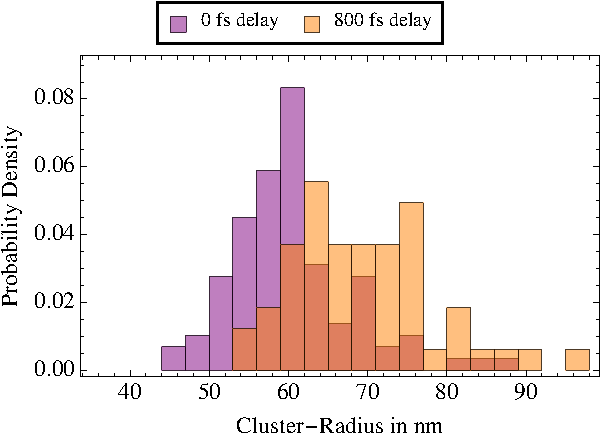
\includegraphics[width=0.75\textwidth]{images/size-distributions.pdf}
	\caption[Single Xe-cluster size distribution at varying time delay $\Delta t$.]{Size evaluation of $\sim 30$ single Xe-cluster hits per time delay $\Delta t$ step. At $\Delta t=0$ fs, the size distribution follows an expected log-normal distribution, while at $\Delta t=800$ fs the distribution broadens and shifts towards larger radii due to the nanoplasma transition.}
	\label{fig:size-distributions}
\end{figure}
In the above mentioned high-throughput size evaluation, Equation \eqref{eq:scattering from sphere} is used to automatically determine the cluster radii of several hundred Xe-clusters. Figure \ref{fig:size-distributions} shows a distribution of cluster radii at X-ray pump--X-ray probe delays, $\Delta t =$ \SIlist{0;800}{\femto\second}. The size distribution of Xe-clusters follows a log-normal distribution \citep{Schutte-2002-IJMS} and at $\Delta t=0$ fs the mean cluster radius is 61 nm. When the delay is increased to $\Delta t=800$ fs, the mean cluster radius increases to 74 nm and the distribution becomes more broad. The mean cluster radius increase by $\sim 20 \%$ over the time delay of 800 fs is attributed to the nanoplasma expansion, as the cluster source should have a stable size distribution. The Xe-cluster size distribution may become more broad due to a distribution of the pump-pulse power density that varies the expansion speed from shot-to-shot.\\[1\baselineskip]
%
Figure \ref{fig:filter-size-intensity} summarizes the mean cluster radii data over several pump--probe delay steps, $\Delta t=$ \SIlist{0;120;250;400;800}{\femto\second}. This data suggests that the nanoplasma expansion speed, $v_{\text{exp}}$, is constant. With the mean cluster radii at $\Delta t=$ \SIlist{0;800}{\femto\second}, we note $v_{\text{exp}}\approx \SI{15250}{\meter\per\second}$. We may use this expansion speed to estimate the electron temperature of the nanoplasma. Here, it is assumed that electrons thermalize with the nucleus within a few femtoseconds such that the velocity distribution of the hot electron gas in the nanoplasma follows a Maxwell-Boltzmann distribution. If we use $v_{\text{exp}}$ as mean velocity of a Maxwell-Boltzmann distribution the electron temperature is $\sim 125$ eV, which compares to temperatures that can be found inside the sun. We can also compare the electron temperature to a similar IR pump--X-ray probe nanoplasma study on Xe-clusters \citep{Gorkhover-2016-NatPho}, where electron temperatures of $\sim 200$ eV have been found. The difference in expansion speed and electron temperature is attributed to the different pump-pulse parameters. Although the IR-pump pulse had power densities of only $\sim 10^{15}$ W cm$^{-2}$ compared to the $\sim 10^{17}$ W cm$^{-2}$ of the X-ray-pump pulse in this study, the X-ray absorption cross-section is much smaller than the IR cross-section. Ultimately, the Xe-clusters absorb more energy from IR-pump pulses than X-ray-pump pulses of similar power density.\\[1\baselineskip]
% NO OF SCATTERER
\begin{figure}
	\centering
		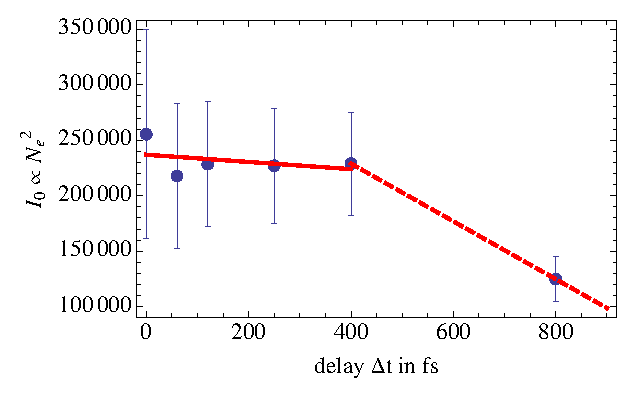
\includegraphics[width=0.80\textwidth]{images/results/number-of-scatterer.eps}
	\caption[Time-resolved behavior of number of scatterers due to nanoplasma expansion]{Intensity $I_{0}$ in arb. units at $\vec{Q}\rightarrow 0$, which is proportional to the total number of scatterers squared $N_{e}^{2}$, here electrons. The data show that the expanding cluster Coulomb traps electrons steadily in the initial stages of the nanoplasma expansion but as the trapping potential decreases due to the multi-step ionization a sudden decrease of $\sim 65\%$ electrons is observed.}
	\label{fig:number-of-scatterer}
\end{figure}
The total number of scatterers, i.e., electrons that interact with the LCLS pump-pulse, is deduced from the diffraction patterns via an intensity analysis. As described in the theory Section \ref{sec:saxs}, when
\begin{equation}
I\left(\vec{Q}\rightarrow 0\right) \propto N_{e}^{2},
\label{eq:}
\end{equation}
where $I$ is the distribution of the scattered intensity as a function of the scattering vector $\vec{Q}$, we can determine the number of electrons, $N_{e}$, that contribute to the scattering process. Figure \ref{fig:number-of-scatterer} shows the parameter $\rho_{0}^{2}$, from Equation \eqref{eq:scattering from sphere}, as a function of the time delay $\Delta t$ (blue dots). As the incident beam intensity, $I_{0}$, remains constant in the X-ray pump--X-ray probe setup $\rho_{0}^{2} \propto N_{e}^{2}$. Two linear fits (red lines) have been added to the figure to visualize the effect. The data show that up to a delay of $\Delta t=400$ fs the amount of electrons $N_{e}$ in the interaction region rather constant (solid red line). However, at a time delay of $\Delta t=800$ fs, the number of scattering electrons decreases on average by $\sim 26 \%$ (dashed red line). This supports the idea that the Coulomb barrier\index{nanoplasma expansion!Coulomb trapping} efficiently traps electrons from the ionization process in the initial stages of the nanoplasma expansion\index{nanoplasma!expansion}, here, up to 400 fs after the pump-pulse. But, eventually, the electrons overcome the trapping potential and dissipate the interaction region, such that they do not contribute to the diffraction image anymore. The key driver that lowers the trapping potential, thus releasing the electrons, is the expansion of the cluster. The effect of trapped electrons has been simulated in, e.g., \citep{Hau-Riege-2004-PRE}. Trapped electrons contribute drastically to the radiation damage process due to secondary collisional ionization.\\[1\baselineskip]
%
In a thought-experiment, where SPI is performed using long X-ray pulses of $\sim 100$ fs, the sample would get ionized and efficiently traps electrons. The trapped electrons can be treated as non-relativistic, thus they do contribute coherently to the scattering pattern. However, their contributions reduce the contrast as their positions are not related to the structure. A similar damage effect is described in \citep{Quiney-2010-NatPhys} and it is shown that computational methods may compensate for such damage.\\[1\baselineskip]
% 2D RECONSTRUCTIONS
\begin{figure}
	\centering
		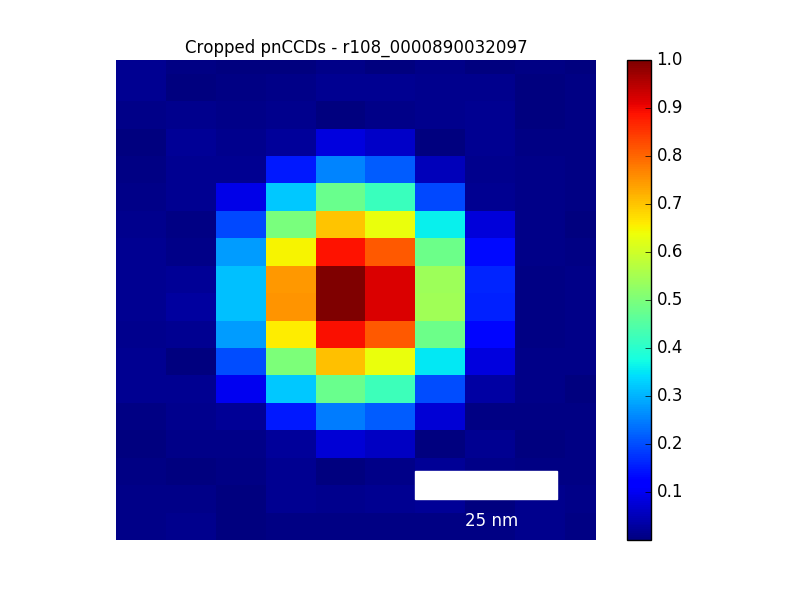
\includegraphics[width=0.49\textwidth]{images/results/Xe_0_fs.png}
		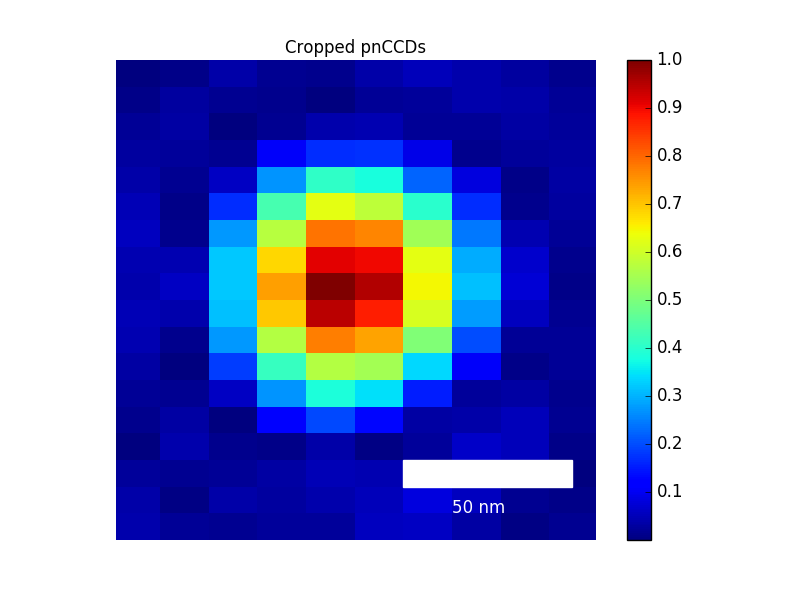
\includegraphics[width=0.49\textwidth]{images/results/Xe_800_fs.png}
	\caption[Single-shot 2D reconstructions of $\sim 25$ nm radius Xe-clusters.]{Single-shot 2D reconstructions of diffraction patterns from single Xe-clusters. The left image shows a $\sim 25$ nm radius Xe-cluster at a pump--probe delay $\Delta t=0$ fs. The cluster has a spherical or arguably icosahedral electron density distribution that is distinct compared to the background. The right image shows a $\sim 25$ nm radius Xe-cluster at a time delay $\Delta t=800$ fs that shows a similar symmetry but due to the loss of scatterers (see fig \ref{fig:number-of-scatterer}), the signal-to-noise ratio decreases and a ringing appears that is likely generated by the support structure in the iterative process.}
	\label{fig:Xe-2D-reconstructions}
\end{figure}
Figure \ref{fig:Xe-2D-reconstructions} shows 2D reconstructions of single Xe-clusters at $\Delta t = 0$ fs in the left panel and $\Delta t=800$ fs in the right panel. The clusters appear generally spherical, however, an icosahedral shape is imaginable. Both clusters have a radius of $r\approx 25$ nm. The reconstructions constitute some of the smallest objects recovered with diffraction imaging at the time of writing. The minimal resolvable feature size in these images is $\sim 14\times \sim \SI{6}{\square\nano\meter}$ along the $X\times Y$-axis (see Section \ref{sec:resolution-discussion}). The reconstruction at $\Delta t=800$ fs shows a ringing around the actual cluster, which is likely an artifact of the spherical support structure. This ringing becomes visible due to a lower signal-to-noise ratio, which is due to the described loss of electrons in the interaction region. Due to the resolution limitation, a nanoplasma expansion, i.e., the earlier discussed \SI{20}{\percent} increase in Xe-cluster radius, may be difficult to see. Also, 2D reconstructions of nanoparticles of that size are challenging and the number of successful 2D reconstructions is low. We thus analyze the xenon imaging data in 1D in the following paragraphs.\\[1\baselineskip]
% 1D RECONSTRUCTIONS
\begin{figure}
	\centering
		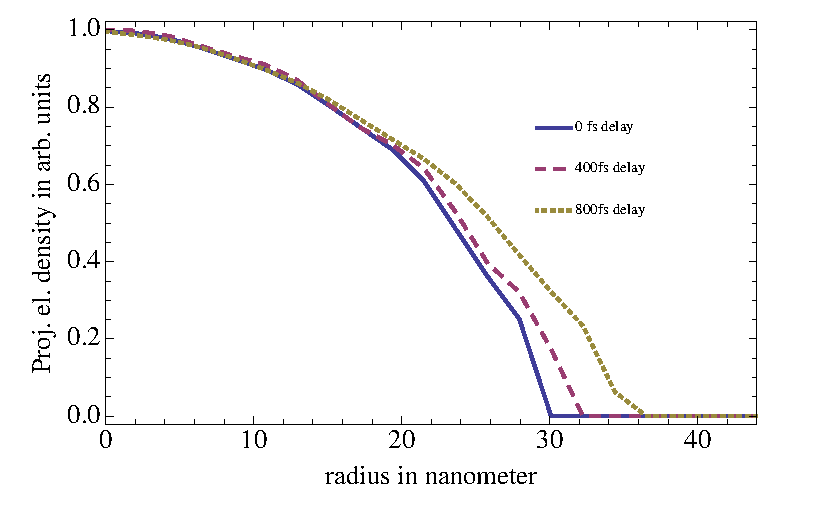
\includegraphics[width=0.80\textwidth]{images/results/Xe-reconstructions.eps}
	\caption[Single-shot 1D reconstruction of $\sim 30$ nm radius Xe-cluster]{Single shot 1D reconstruction of Xe-cluster at various time delays $\Delta t$. The figure shows the projected and normalized el. mass as a function of the radius, i.e., the electron density. These real-space images of a nanoplasma transition show that, at first, outer atomic layers are shed off, here imaged at $\Delta t=400$ fs. And over time, more inner atomic layers follow, here imaged at $\Delta t= 800$ fs.}
	\label{fig:Xe-reconstructions}
\end{figure}
%TO MOVE ON 1D reconstructions of single xenon cluster were obtained as described in Section \ref{sec:1d-proj-and-phase-reconstruction}. Figure \ref{fig:Xe-reconstructions} shows 1D reconstructions of the projected electron density from single xenon cluster at time delays $\Delta t=\{0, 400, 800\}$ fs between the X-ray pump and X-ray probe beam. The density curves are normalized to clearly indicate an expansion of the outer atomic layers of the cluster. In this selection of hits, the cluster radii expand by $\sim 20\%$ over a time delay of $\Delta t=800 fs$, which is a substantial structural change. To make these events COMPARABLE INCLUDE DIFFRACTION PATTERNS. ELECTRON TEMPERATURE\\
Real-space images of single Xe-clusters have been recovered in 1D in Figure \ref{fig:Xe-reconstructions} (see methods Section \ref{sec:1d-proj-and-phase-reconstruction}). The 1D reconstructions show normalized and projected electron density from single xenon cluster at time delays $\Delta t=$ \SIlist{0;400;800}{\femto\second}. At $\Delta t = 0$ fs, the electron density follows the density projection of a sphere (compare Figure \ref{fig:cluster-generation}). With a delay of $\Delta t = 400$ fs, an expansion of the outer atomic layers of the cluster is observed. At $\Delta t = 800$ fs, outer layers continue to expand and inner atomic layers start to follow. Over the time delay sequence $\Delta t=0$ to $800$ fs, the cluster radius expands $\sim 20\%$, or from $r\approx 30$ nm to $r\approx 36$ nm. This sequence of events gives insight into the shape of the Xe-cluster as it undergoes the nanoplasma transition and directly confirms theoretical predictions, e.g., \citep{Hau-Riege-2004-PRE}. The images clusters have comparable initial sizes as they are selected from the lower end of the cluster size distribution.\\[1\baselineskip]
% AMPLITUDE AND PHASE DISCUSSION
\begin{figure}
	\centering
		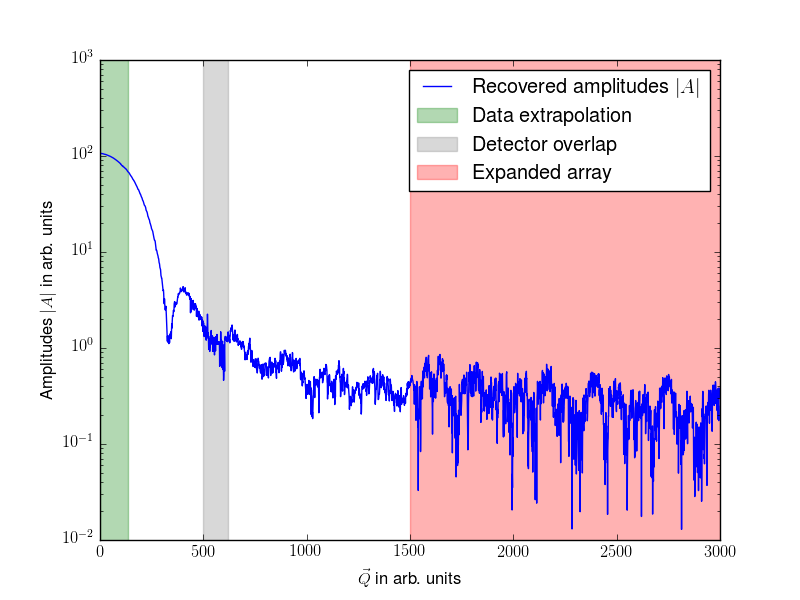
\includegraphics[width=0.49\textwidth]{images/results/amplitude-discussion.png}
		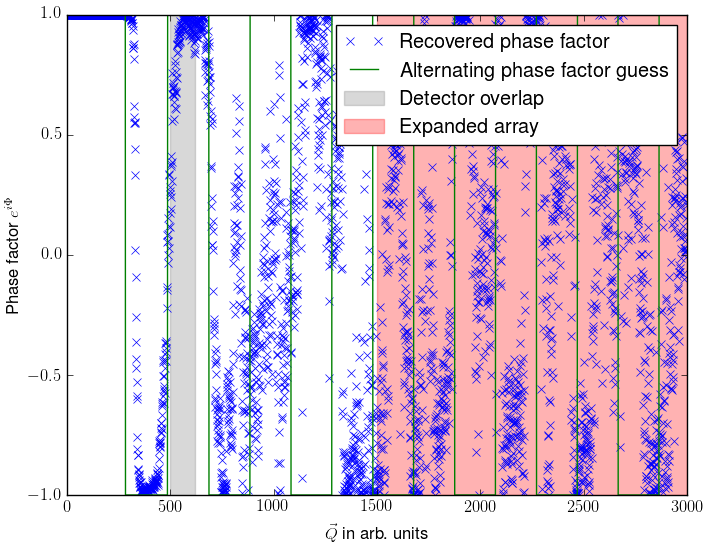
\includegraphics[width=0.49\textwidth]{images/results/phase-discussion.png}
	\caption[Recovered Amplitudes $\left|A\right|$ and phase factor of 1D reconstruction]{The left panel shows the recovered amplitudes $\left|A\right|$ and the right panel shows the phase factor of the 1D phase retrieval. The green and red background indicates the space where initial data points were extrapolated. The gray area discloses the detector overlap. See Section \ref{sec:1d-proj-and-phase-reconstruction} for more details.}
	\label{fig:amplitude-phase}
\end{figure}
For the sake of completeness of these 1D reconstructions, the recovered modulo of the amplitude, $\left|A\right|$, and the recovered phase factor are shown in Figure \ref{fig:amplitude-phase} for the data at $\Delta t =800$ fs. The amplitudes $\left|A\right|$ have been replaced in the space with white background. The data with the green background was interpolated using the anticipated scattering of a sphere. The grayed area indicates the pnCCD detector overlap and the red background data is extrapolated from the scattering of a sphere. The red area therefore increases the resolution. The data points of the k-times iterated Fourier-space function $G'_{k}(\vec{Q})$ in the white area were replaced with the original data set while $G_{k}(\vec{Q})$ was allowed to evolve freely in the remaining area. The phase factor retrieval starts with an initial guess of alternating signs per diffraction ring of the sphere and then evolves freely. One can see how the recovered phase factor is alternating as one would expect from the scattering of a sphere.\\[1\baselineskip]
% SINGLE SHOT DIFF PATTERN
\begin{figure}
	\centering
		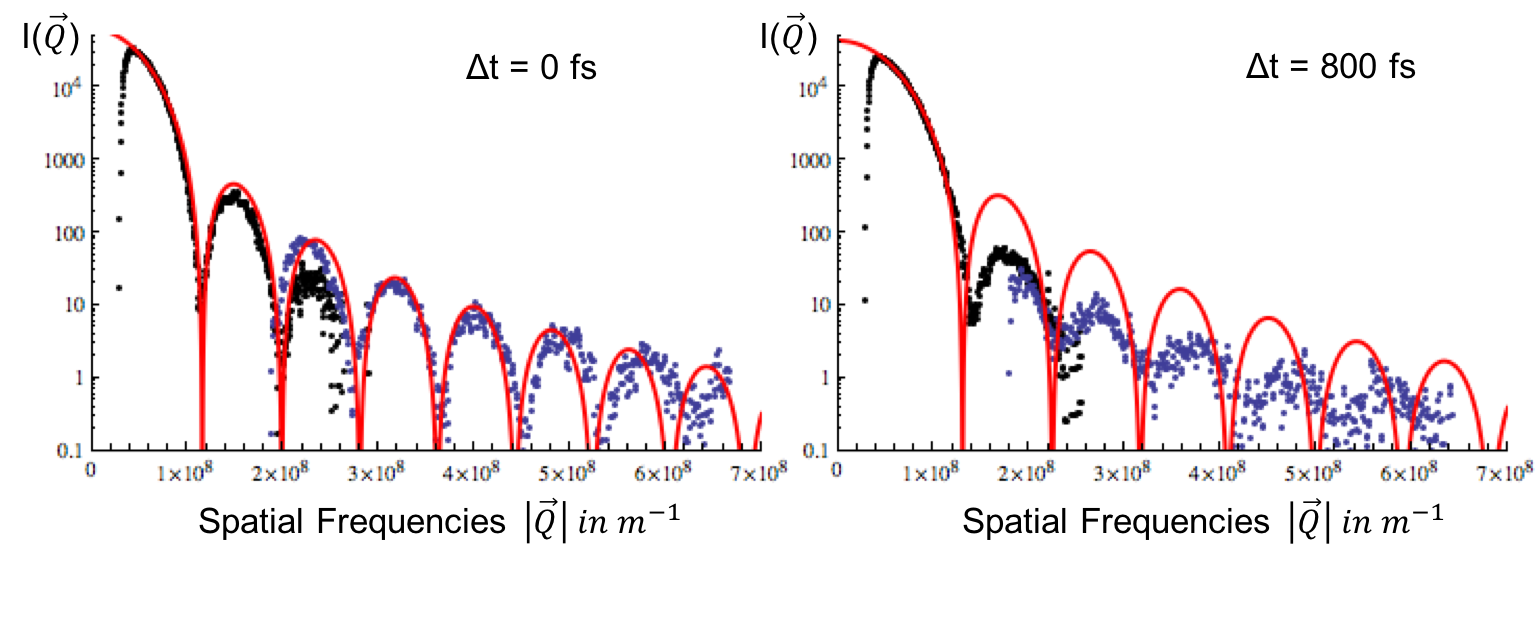
\includegraphics[width=1.0\textwidth]{images/results/Xe-diff-pattern.png}
		%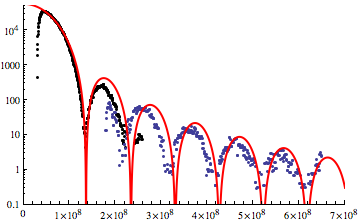
\includegraphics[width=0.49\textwidth]{images/results/Xe-only-60fs.png}\\
		%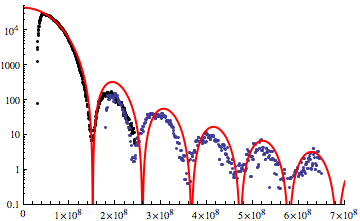
\includegraphics[width=0.49\textwidth]{images/results/Xe-only-120fs.png}
		%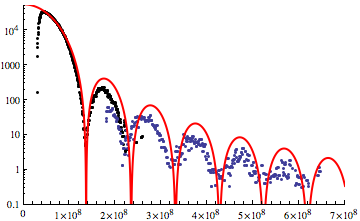
\includegraphics[width=0.49\textwidth]{images/results/Xe-only-250fs.png}\\
		%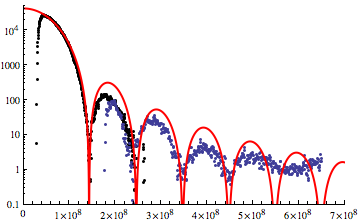
\includegraphics[width=0.49\textwidth]{images/results/Xe-only-400fs.png}
		%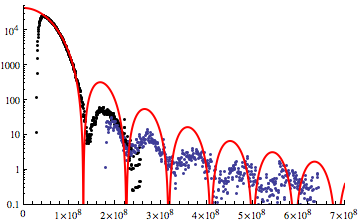
\includegraphics[width=0.49\textwidth]{images/results/Xe-only-800fs.png}
	\caption[Single-shot diffraction pattern of Xe-cluster at varying time delays]{Single shot diffraction pattern at certain pump--probe delays $\Delta t$. The red curve simulates the scattering of a sphere, the black data points are from the rear pnCCD detector and the blue data points are from the front pnCCD. The nanoplasma expansion manifests in the scattering intensity $I$ at large spatial frequencies $\left|\vec{Q}\right|$, where $I$ decreases as described in \citep{Gorkhover-2016-NatPho}.}
	\label{fig:Xe-only-diff-pattern}
\end{figure}
We may also analyze the Xe-cluster in reciprocal space and analyze the radial projections of the measured diffraction patterns directly. Radial projections of single-shot diffraction patterns from single Xe-cluster can be found in Figure \ref{fig:Xe-only-diff-pattern}. The figure shows a red line, which is the scattering from a sphere as per Equation \eqref{eq:scattered-intensity} and \eqref{eq:scattering from sphere} fitted onto the low-$\left|\vec{Q}\right|$ signal of the zeroth diffraction scattering order using the radius and the incident beam intensity variable. The black data points are projected from the rear pnCCD and the blue data points are projected from the front pnCCD using the projection method described in \ref{sec:combination-of-images}. At $\Delta t=0$ fs, the scattering of the Xe-cluster can be well approximated with the scattering of a sphere. Hence, the fit (red line) agrees well with the data points up to scattering angles of $\Theta \approx 9$° or $\left|\vec{Q}\right|\approx\SI{6.8e8}{\per\meter}$. However, it should be noted that this comparison becomes less good at very large scattering angles due to the flat detector \citep{Bostedt-2012-PRL} and deviations in the diffraction pattern from a perfect sphere. As the time delay $\Delta t$ increases, the large-$\left|\vec{Q}\right|$ scattering signal decreases and the scattering of a plain sphere does not fit the scattering well anymore. A similar effect is also observed in the previously mentioned IR pump--X-ray probe study \citep{Gorkhover-2016-NatPho}. Due to the nanoplasma transition, the Xe-cluster is expanding with the outer layers expanding faster than the core. A mathematical description of this damage model, namely an expanding sphere, has been introduced in Section \ref{sec:2d-simulations}. It generally fits the data well, as it is shown in great detail in \citep{Gorkhover-2016-NatPho,Gorkhover-2014-Thesis}. Note that the X-ray pump--X-ray probe considerations from Section \ref{sec:pump--probe-considerations} would minimize the effect of a decreased scattering at large scattering angles.
%
%
%
\section{Time-dependent response of Xe-atoms due to an X-ray pump--probe beam}\label{sec:time-resolved-xe-atoms}
%%%%%%%%%%%%%%%%%%%%%%%%%%%%%%%%%%%%%%%%%
%- Xe iToF dynamics\\
%- Slightly more of Xe higher charge-states present at longer delays.
%%%%%%%%%%%%%%%%%%%%%%%%%%%%%%%%%%%%%%%%%
\begin{figure}
	\centering
		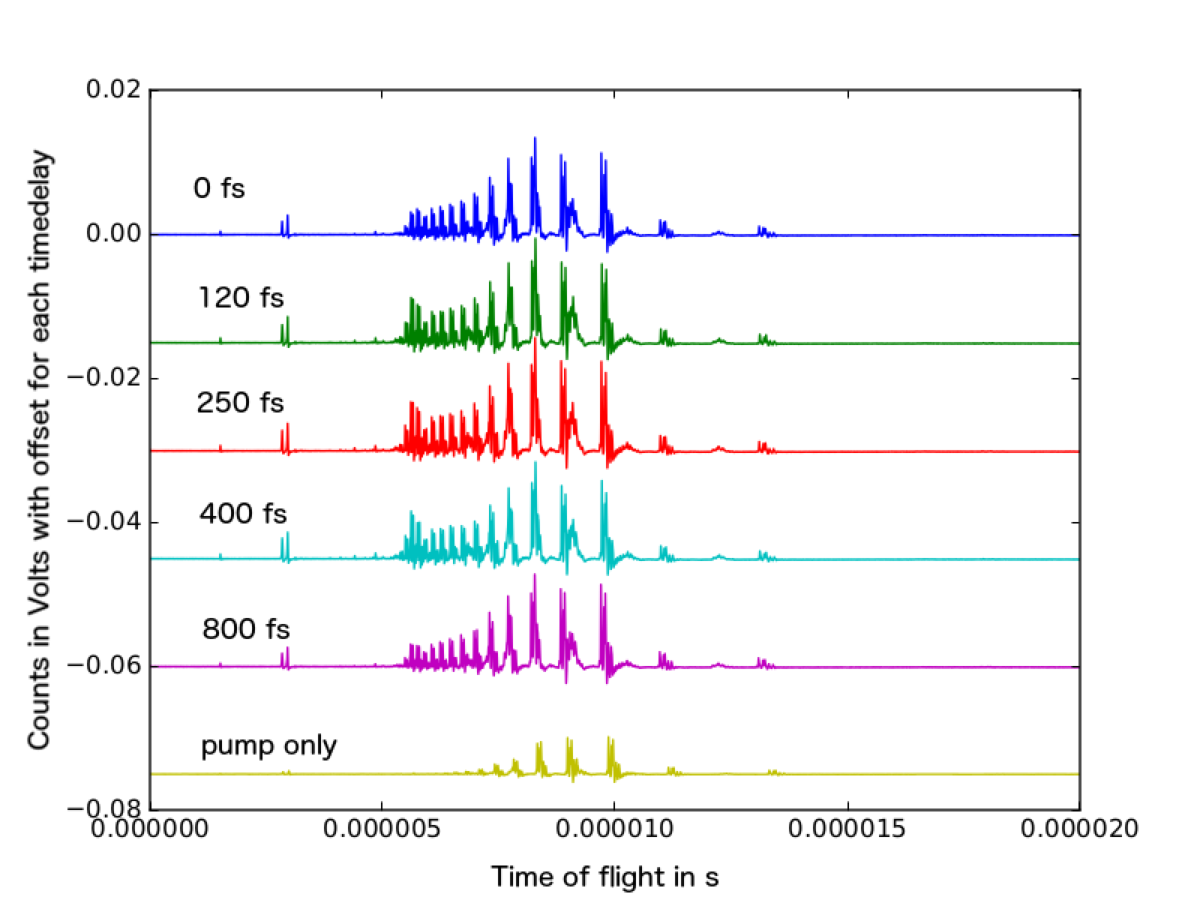
\includegraphics[width=0.49\textwidth]{images/results/TOF-atomic-xenon.png}
		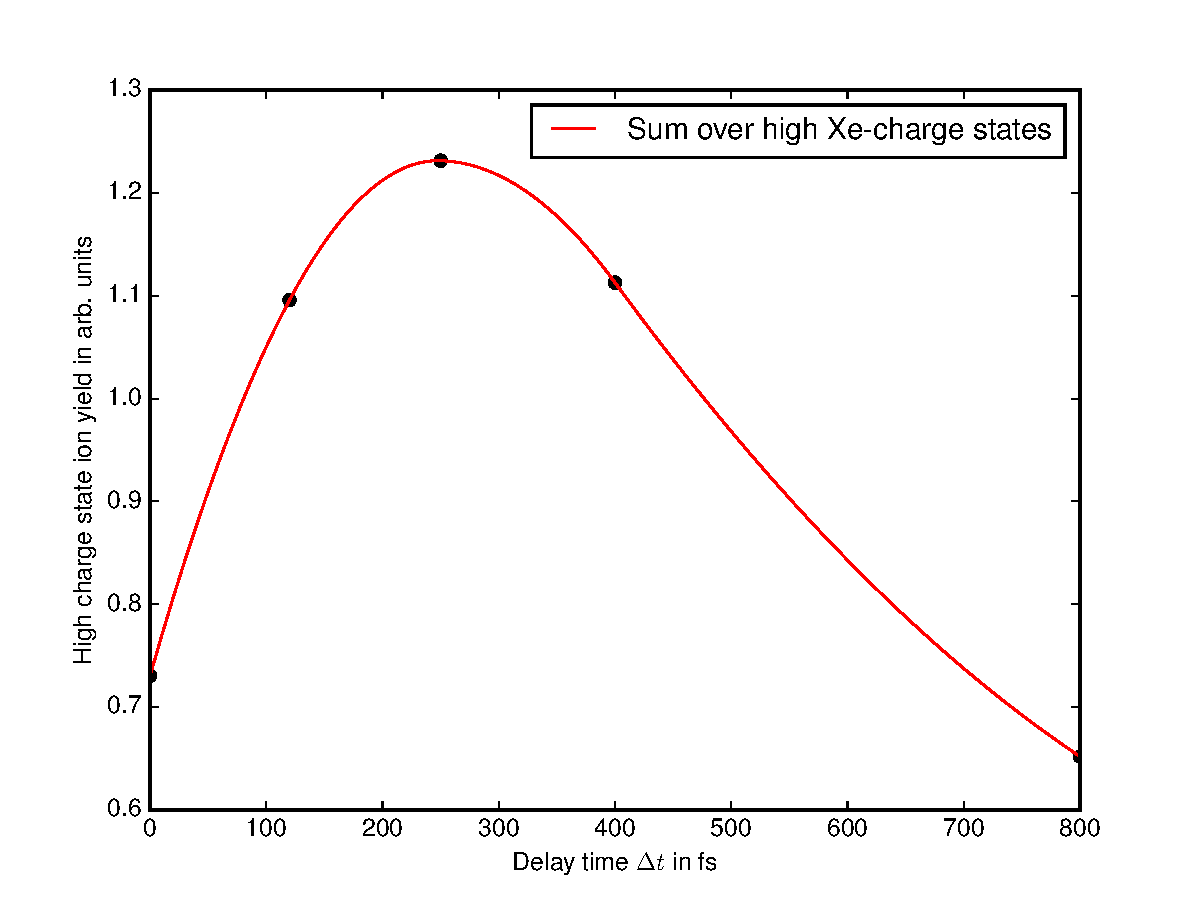
\includegraphics[width=0.49\textwidth]{images/results/atomic-charge-state-time-resolved.pdf}
	\caption[Time-resolved answer of atomic xenon in TOF spectroscopy.]{Atomic xenon ion time-of-flight data shows resonant type behavior. As the X-ray pump-pulse traverses through the xenon ions, the 3d-subshell becomes highly ionized and thus the atom becomes increasingly transparent for the probe-pulse ($\Delta t \approx 0-120$ fs). The electron-holes have a longer lifetime due to the highly ionized subshell. After the Auger decay populates the 3d-subshell, the atom becomes less transparent and the X-ray probe-pulse efficiently ionizes the atoms ($\Delta t \approx 250$ fs). Eventually, relaxation processes dissipate energy leading to fewer high-charge states.}
	\label{fig:TOF-atomic-xenon}
\end{figure}
Ion time-of-flight traces of atomic xenon at different time delays $\Delta t =$ \SIlist{0;120;250;400;800}{\femto\second} and X-ray pump-pulse only data is shown in Figure \ref{fig:TOF-atomic-xenon}. The time-of-flight data show a resonance behavior as the atomic xenon high-charge states peak at $\Delta t = 250$ fs. The xenon high-charge states start low at $\Delta t = 0$ fs and then peak due to intensity-induced X-ray transparency \citep{Young-2010-Nature,Schorb-2012-PRL}. In the present study, the xenon 3d-subshell is efficiently ionized by the X-ray pump-pulse. These electron-holes are typically repopulated on the few femtosecond timescale due to the Auger decay, however, the increasingly ionized atom has longer electron-hole lifetimes and the Xe-atoms become increasingly transparent as the X-ray pulse propagates. It has been measured that $\text{Ne}^{8+}$ has core-hole lifetimes of $~230$ fs. But why does the charge state distribution then not level out for later delays $\Delta t > 250$ fs? When the strongly pumped atom does not absorb energy near saturation, relaxation processes catch up and effectively dissipate energy, thus reducing the average ionization level.
%\begin{figure}
	%\centering
		%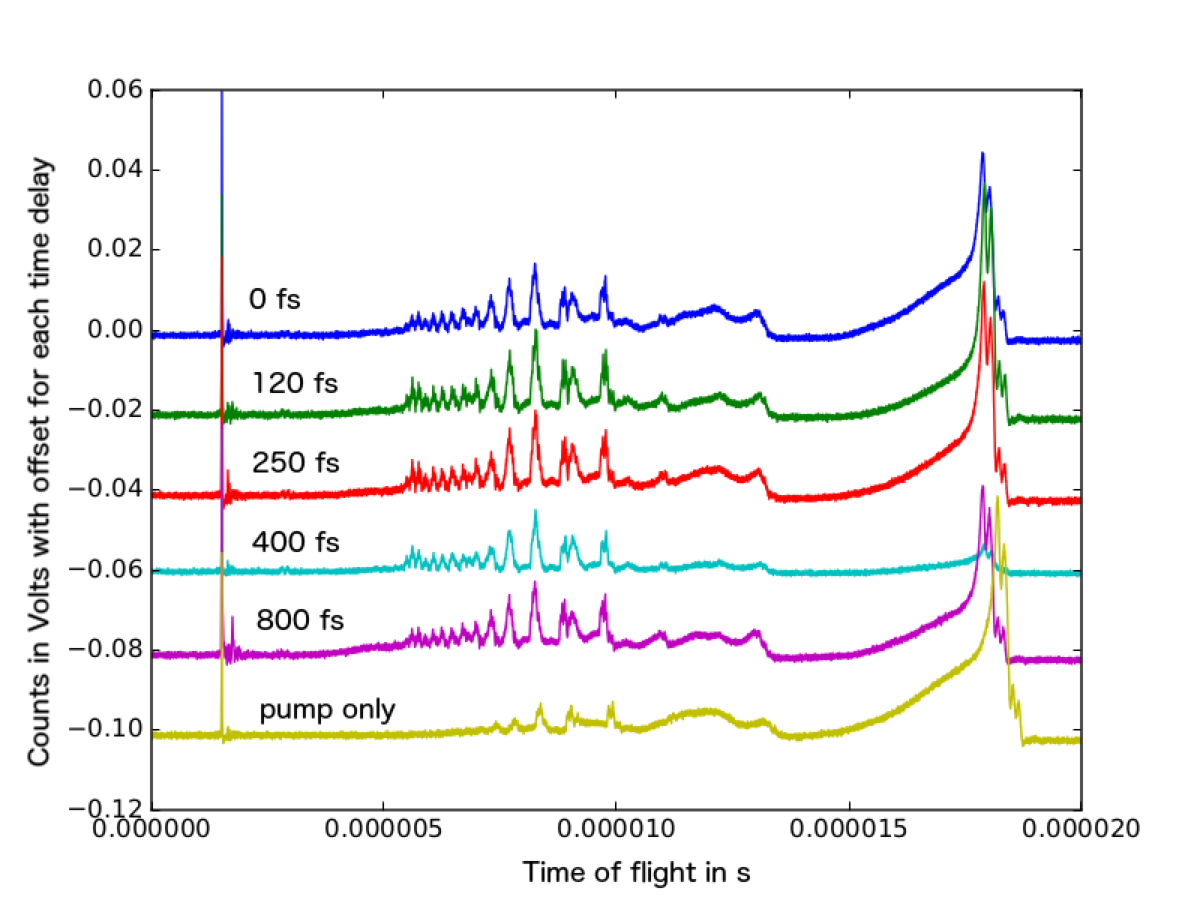
\includegraphics[width=0.80\textwidth]{images/results/TOF-small-cluster-xenon.png}
	%\caption{caption}
	%\label{fig:TOF-small-cluster-xenon}
%\end{figure}
%Figure \ref{fig:TOF-small-cluster-xenon} shows ion time-of-flight traces of small xenon cluster cluster at different time delays $\Delta t = \{0,120,250,400,800\}$ fs and X-ray pump only data. To create xenon cluster on the order of XXX nm radius the reservoir pressure in the source has been changed to $p_{0}=6$ bar. The data show similar resonant behavior as in the atomic case. Xenon high-charge states peak at an X-ray pump--X-ray probe delay of 250 fs and start decrease at higher delays. At longer time-of-flight durations of 10 $\mu$s and beyond the small cluster signal dominates. Due to the short run times, the fluctuations of the cluster source vary the cluster signal significant.\\
%\begin{figure}
	%\centering
		%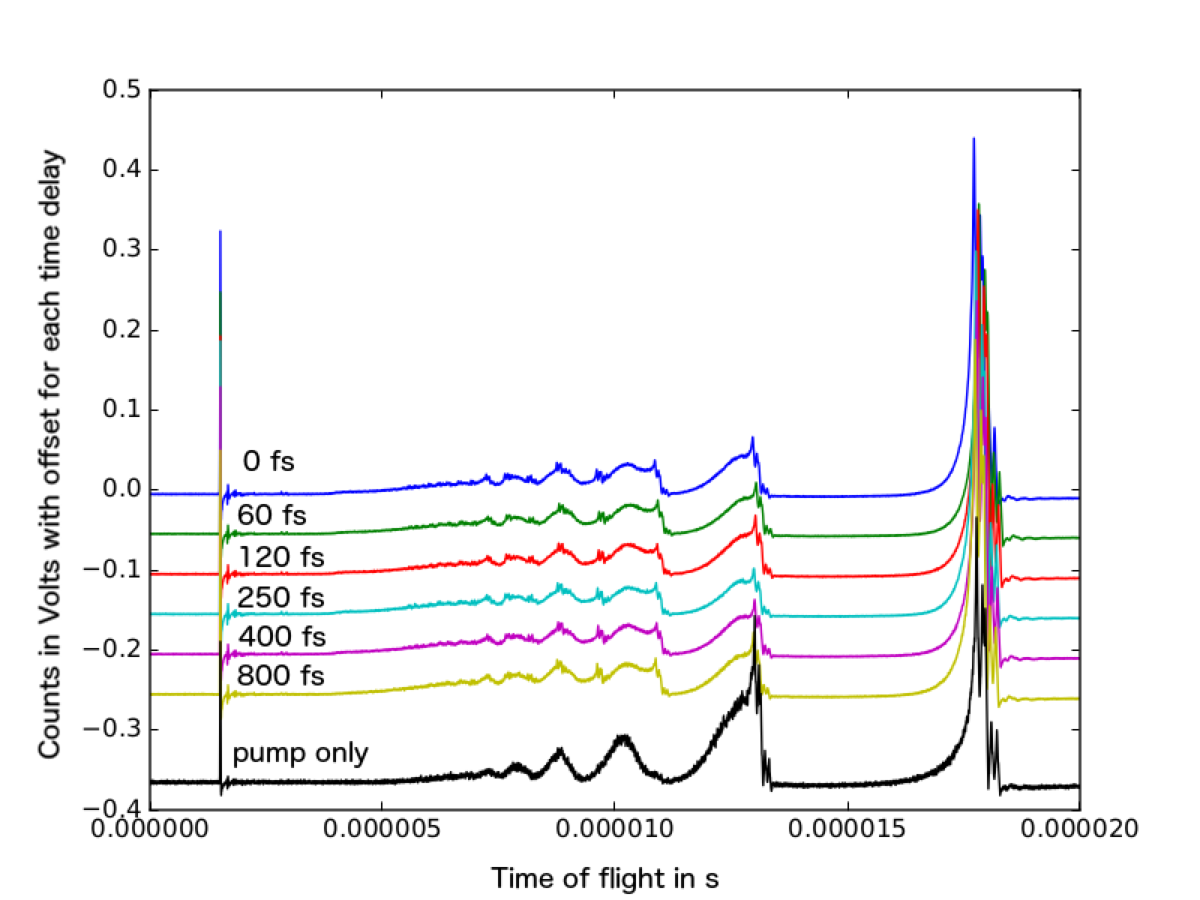
\includegraphics[width=0.80\textwidth]{images/results/TOF-regular-cluster-xenon.png}
	%\caption{caption}
	%\label{fig:TOF-regular-cluster-xenon}
%\end{figure}
%Ion time-of-flight traces of larger clusters can be found in Figure \ref{fig:TOF-regular-cluster-xenon}. Here a mean Xe-cluster radius of $\sim 61$ nm is observed. The time delay between X-ray pump and X-ray probe has been set to $\Delta t=\{0,60,120,250,400,800\}$ and also the pump only data is shown. The data show that the cluster type of signal is dominating the trace. At a time delay $\Delta t=800$ fs, the xenon high-charge states increase, while no other dynamic appears obvious from the average data. The larger cluster ensemble may undergo a similar resonant type behavior as atomic xenon, however, the large cluster ensemble seem to affect the ionization pathways and thus the timescale of the resonant type behavior.\\
%Summarizing, atomic xenon, xenon cluster of mean radius $\sim XXX$ nm and Xe-cluster of average radius $\sim 61$ nm were investigated using an X-ray pump--X-ray probe setup coincidently measuring spectroscopy and coherent diffractive imaging data. The ion spectroscopy data of atomic xenon high-charge states show a resonant type behavior as the time delay $\Delta t$ is varied from 0 fs to 800 fs. The effect peaks, i.e. is resonant around 250 fs. Small xenon cluster exhibit a similar behavior as atomic signal because atomic signal is dominating the high-charge states. The signal from larger xenon cluster of radii $\sim 61$ nm is dominated by xenon charge fragments. An increase in the xenon high-charge states is observed at 800 fs, allowing us to conclude that the ionization dynamics have changed. It is interesting to note that altough larger cluster absorb overall more energy, the ensemble of atoms that is bound in the cluster is able to collectively change, here slow, ionization pathways. This behavior may be reproduced in other nano-samples such as bio-molecules or artifical tamper layers.
%
%
%
%%%%%%%%%%%%%%%%%%%%%%%%%%%%%%%%%%%%%%%%
\section[Time-resolved response of highly ionized He- and HeXe-clusters]{Time-resolved response of highly ionized He-clusters and xenon doped He-clusters}\label{sec:hexe--and-he-TOF}
%%%%%%%%%%%%%%%%%%%%%%%%%%%%%
% - Subsection for iToF data, important to compare to HeXe data.
%%%%%%%%%%%%%%%%%%%%%%%%%%%%%
\begin{figure}
	\centering
		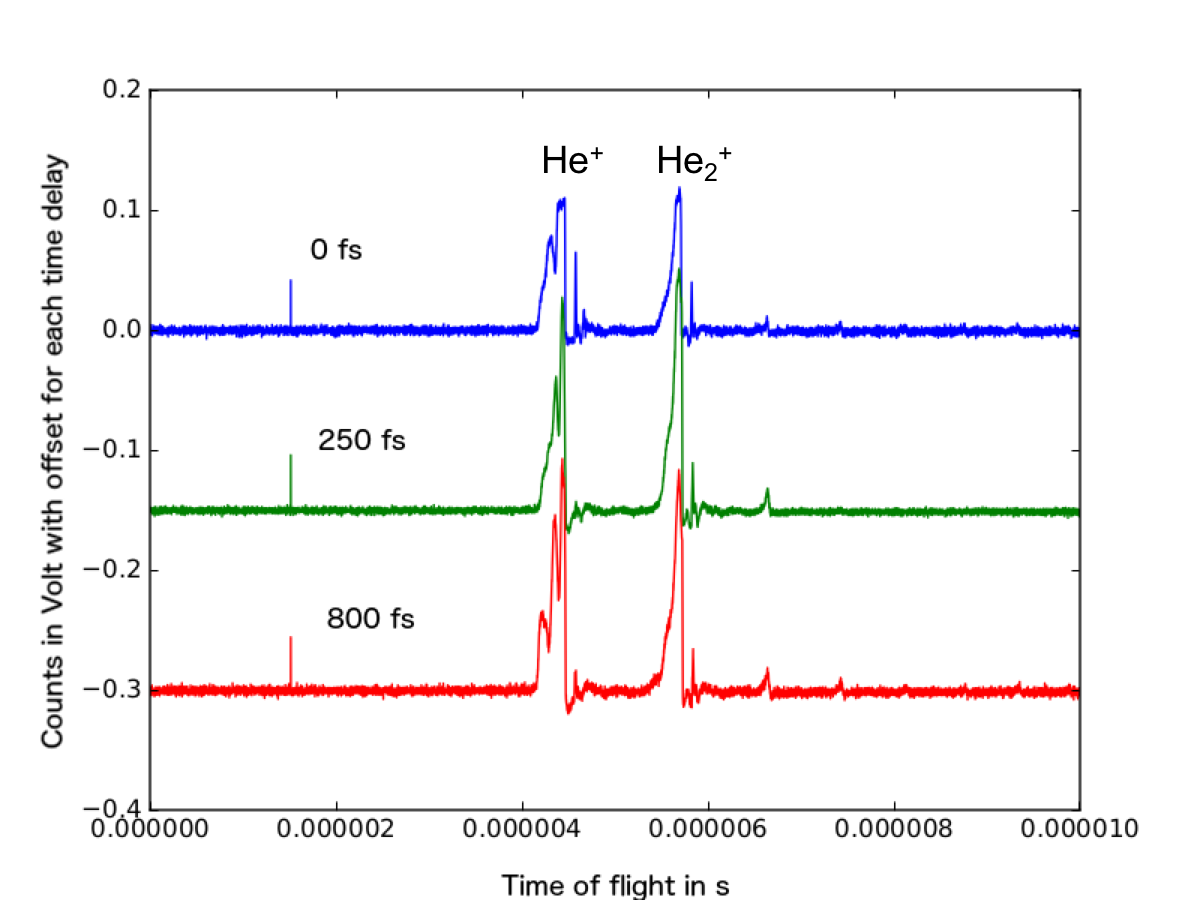
\includegraphics[width=0.65\textwidth]{images/results/TOF-helium-cluster.png}
	\caption[Time-resolved answer of He-clusters in TOF spectroscopy.]{Ion time-of-flight traces of He-cluster with a radius of $r_{\text{He}}\approx 810$ nm. Although minor changes in the charge fragmentation are observed, we shall note that there are no $He^{2+}$ ions in this data. The absorption cross-section of helium are too low to lead to doubly-charged states \citep{Ho-2016-PC}.}
	\label{fig:TOF-helium-cluster}
\end{figure}
The response of clusters in highly intense X-ray radiation is more complex than the atomic signal. Size-dependent \citep{Schorb-2012-PRL,Schutte-2015-JPhysB} and recombination effects in the nanoplasma \citep{Schutte-2014-PRL} alter the sample's ionization pathways. Figure \ref{fig:TOF-helium-cluster} shows ion time-of-flight data of pristine He-cluster charge fragments at pump--probe delays $\Delta t=$ \SIlist{0;250;800}{\femto\second}. The pristine He-droplets have a radius of $r_{\text{He}}\approx 810$ nm or $\left\langle N_{\text{He}}\right\rangle\approx 5\cdot 10^{10}$ on average using the relation \citep{Gomez-2011-JCP}
\begin{equation}
r_{\text{He}}=0.22 (N_{\text{He}})^{\frac{1}{3}}\ [\text{nm}].
\end{equation}
The data show an overall similar behavior regardless of the delay $\Delta t$, although minor changes in the charge fragmentation distribution can be seen. More importantly for referencing purposes, the traces indicate no contribution of doubly-charged helium atoms. The lack of double-charged helium can be explained by the comparably low absorption cross-sections of helium (see Table \ref{tab:helium-xenon-ionization}) \citep{Ho-2016-PC}.\\[1\baselineskip]
\begin{figure}
	\centering
		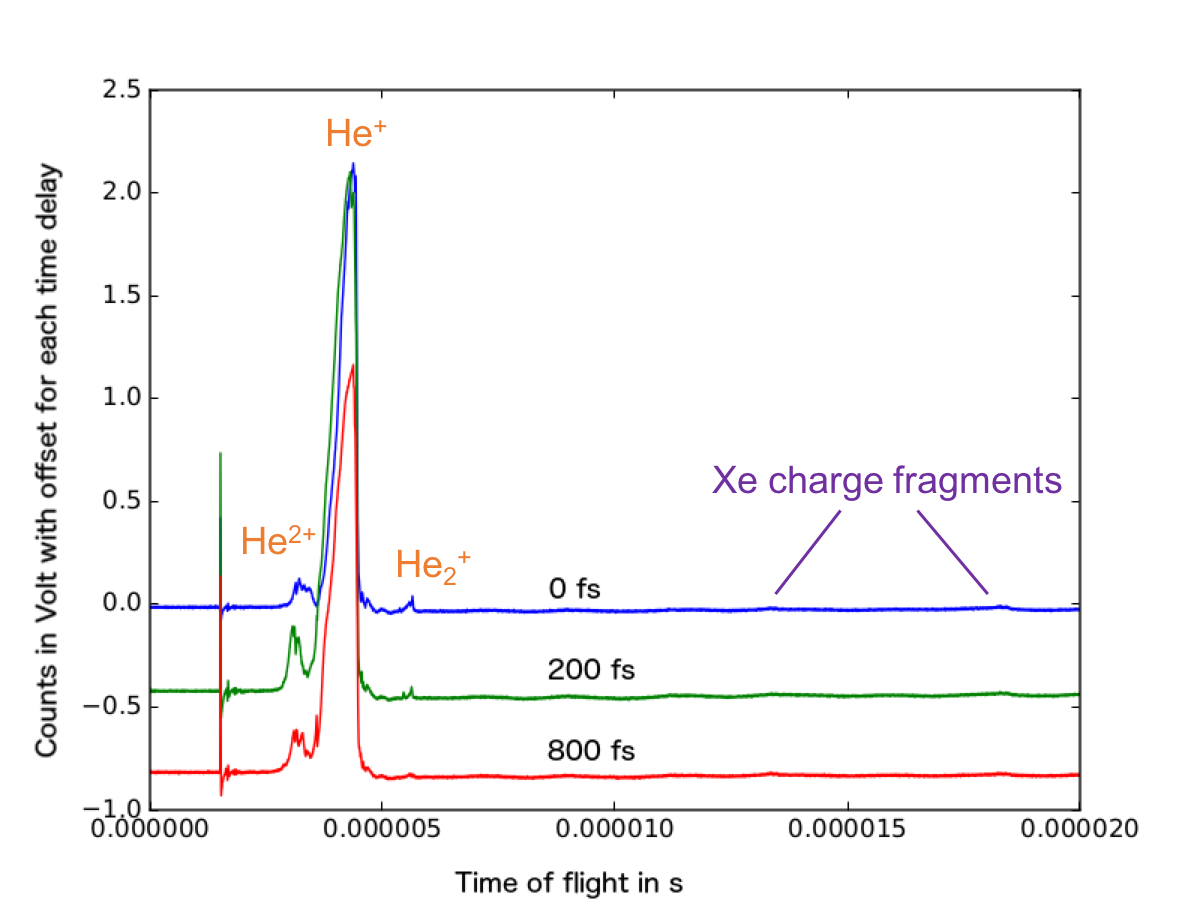
\includegraphics[width=0.65\textwidth]{images/results/TOF-helium-xenon-cluster-60.png}
	\caption[TOF spectra of HeXe-clusters with $\sim 0.6\%$ Xe-doping at various delays $\Delta t$.]{Ion time-of-flight spectra of He-cluster with $r_{\text{He}}\approx 600$ nm radius and Xe-doping levels of $\sim 0.6\%$. The Xe-atoms absorb X-rays efficiently and transfer the absorbed energy to the He-atoms. The Xe-ions recombine and only a few xenon charge fragments are observed. Due to the energy transfer, doubly-charged He-ions are detected and the \textit{kinetic energy release} is increased as well. As the delay time, $\Delta t=$ \SIlist{0;200;800}{\femto\second}, is varied sequentially, the system undergoes a resonant type behavior that is attributed to the ionization dynamics of Xe-atoms.}
	\label{fig:TOF-helium-xenon-cluster-60}
\end{figure}
Xenon doped helium cluster time-of-flight traces are shown in Figure \ref{fig:TOF-helium-xenon-cluster-60}. Here the He-droplets have a radius of $r_{\text{He}}\approx 600$ nm or $\left\langle N_{\text{He}}\right\rangle\approx 2\cdot 10^{10}$ particles with a $\sim 0.6\%$ doping level of xenon. For the sake of completeness, the helium depletion at this doping level is $\sim 62\%$ (see Section \ref{sec:heterogeneous-cluster}). Most notable is the presence of $\text{He}^{2+}$ ions and a strongly increased signal from $\text{He}^{+}$ ions. But, few xenon charge fragments are observed. This is counter-intuitive as the absorption cross-section from xenon is vastly higher than from helium (see Table \ref{tab:helium-xenon-ionization}). We can therefore hypothesize two points. One, there must be an efficient, ultrafast energy transfer process from the Xe-particles to the He-droplet; two, that the helium atoms function as electron reservoir as the initially photoionized xenon atoms must recombine with trapped electrons to be neutrally charged and thus not detected by the ion TOF. As the time delay $\Delta t$ is varied, we observe that the He-ion signal shows a resonant behavior. At $\Delta t = 200$ fs, the signal from $\text{He}^{2+}$ and $\text{He}^{+}$ peaks. However, the helium signal is less intense at the delay times $\Delta t = 0$ and 800 fs. We can make use of the earlier discussion around the data shown in Figure \ref{fig:TOF-helium-cluster} and \ref{fig:TOF-atomic-xenon} and conclude that this behavior does not originate from the absorption and ionization dynamics of the He-droplet but rather from the Xe-atoms with wich the He-droplet is doped. In a theoretic study of HeXe-clusters using optical laser pulses a similar resonant behavior is found \citep{Mikaberidze-2008-PRA}.\\[1\baselineskip]
%Comparing the data from Figure \ref{fig:TOF-helium-cluster} and \ref{fig:TOF-helium-xenon-cluster-60} allows us to conclude that xenon cluster transfer energy to the helium cluster that they are embedded in. This process is very efficient since the resonant behavior that origins from the xenon atoms is constituted in the helium signal, while the xenon signal steadily decreases. Therefore,  This behavior is similar to \citep{Hoener-2008-JPB} but differs in it's geometric arrangement.\\
\begin{figure}
 	\centering
 		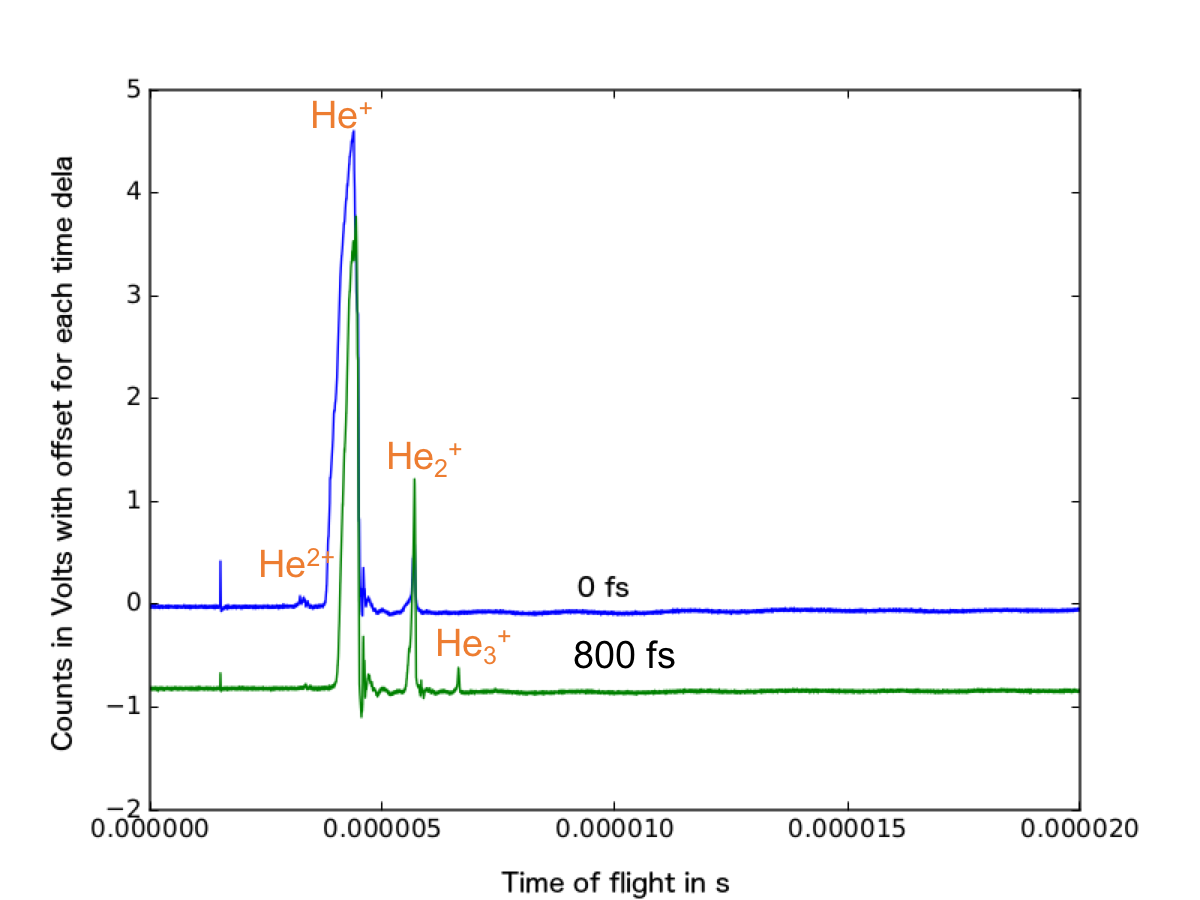
\includegraphics[width=0.65\textwidth]{images/results/TOF-helium-xenon-cluster-13.png}
 	\caption[TOF spectra of HeXe-clusters with $\sim 0.06\%$ Xe-doping at various delays $\Delta t$.]{Ion time-of-flight spectra of He-cluster with $r_{\text{He}}\approx 775$ nm radius and $\sim 0.06\%$ xenon doping. These weaker doped HeXe-clusters show a lower He-ion count and kinetic energy release due to overall less absorption from the lower xenon doping. However, $\text{He}^{2+}$, which indicates an energy transport from the xenon to the helium, is still observed.}
 	\label{fig:TOF-helium-xenon-cluster-13}
\end{figure}
Figure \ref{fig:TOF-helium-xenon-cluster-13} shows ion time-of-flight data of with $r_{He}\approx 775$ nm He-droplets and a $0.06 \%$ doping at pump--probe delays $\Delta t=$ \SIlist{0;800}{\femto\second}. Here, the helium depletion is measured to be $\sim 13\%$. We note, again, the presence of $\text{He}^{2+}$ ions and more signal from $\text{He}^{+}$ ions. However, compared to the higher doped data these peaks are less intense. Qualitatively this can be explained with the less strong xenon doping. The X-ray absorption from the xenon atoms and subsequent energy transfer to the helium atoms dominate the helium ion characteristics, although the He-droplet is larger in this case. So, less doping results in fewer photon absorption processes and thus less energetic helium ion characteristics. Again, at different time delays $\Delta t$, the height of each peak shifts. The $\text{He}^{2+}$ and $\text{He}^{+}$ states become less frequent but a stark increase in $\text{He}_{2}^{+}$ and $\text{He}_{3}^{+}$ ion peaks is observed. It is likely that the ionization dynamics undergo a resonant type behavior, however, there are too few data points to support this hypothesis.\\[1\baselineskip]
%
Summarizing, pristine He-droplets show few dynamics as the time delay $\Delta t$ is varied and only singly-charged $\text{He}^{+}$ ions are measured. If the He-droplets are doped with xenon, doubly-charged $\text{He}^{2+}$ ions are detected, the kinetic energy release is stronger and the time-of-flight data reveals dynamics that are comparable to atomic xenon, when the delay $\Delta t$ is varied. As the xenon doping is increased, the presence of $\text{He}^{+}$ and $\text{He}^{2+}$ ions is more frequent. This data suggests an ultrafast and efficient energy transfer from the xenon atoms to the helium atoms. Collisions could drive this transfer. The helium particles furthermore act as an electron reservoir. The initially photoionized xenon atoms recombine and only few xenon charge fragments are detected by the time-of-flight spectrometer. The underlying idea that a low-Z material acts as a electron supplier for the high-Z material has also been studied in \citep{Hoener-2008-JPB}.
%
%
%
\section{Condensation of xenon in helium cluster: Plum-pudding type cluster}\label{sec:helium-data}
%%%%%%%%%%%%%%%%%%%%
% - Presentation of He data
%%%%%%%%%%%%%%%%%%%%%%%%%%
It is not well known how heterogeneous helium-xenon clusters form a core-shell system. As described in Section \ref{sec:heterogeneous-cluster}, the superfluid helium cluster picks up xenon atoms as it traverses the doping unit. The xenon atoms move unhindered in the superfluid helium and eventually the xenon atoms condense to energetically favorable cluster structures. \citep{Gomez-2014-Science} reports that at a doping level of $0.02\%$, i.e., when there are 5000 more helium atoms than xenon atoms, multiple smaller clusters form and locate at vortexes within a rotating helium droplet. However, it is unknown how xenon atoms arrange in non-rotating droplets and also at higher doping levels. The two competing hypotheses are; one, xenon atoms condense to one large cluster within a helium droplet; two, multiple smaller Xe-clusters form within a droplet. Let us call hypothesis two a \textit{plum pudding core-shell system}\footnote{The name plum-pudding model comes from J.J. Thomson's model of the atom in 1904 and has here been reused to describe the arrangement of atoms in heterogeneous (rare-gas) clusters.} that we can further divide into a case of few and larger scatterers, or many and smaller scatterers.\\[1\baselineskip]
\begin{figure}
 	\centering
 		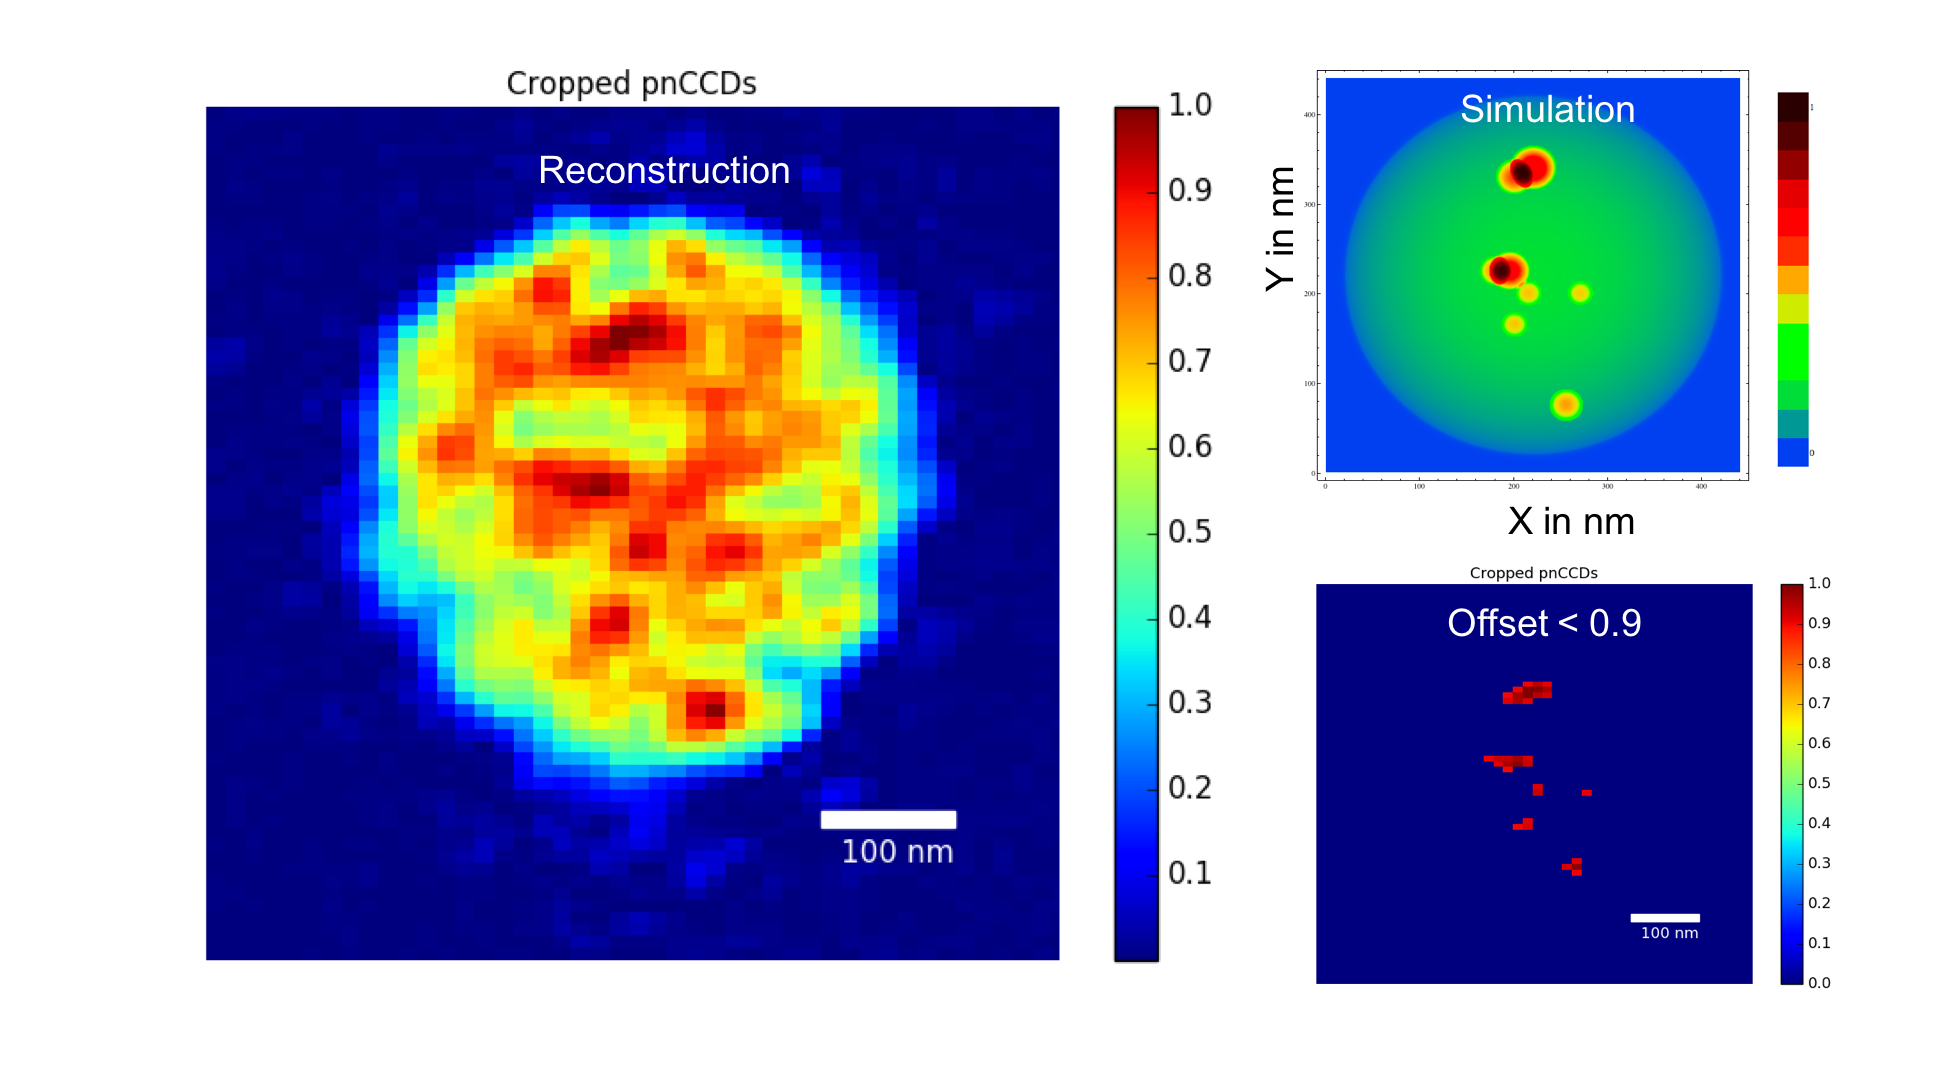
\includegraphics[width=0.80\textwidth]{images/results/reconstructions-to-simulations.png}
 	\caption[Reconstruction of HeXe-clusters and simulated electron densities.]{Real-space reconstruction of a HeXe-cluster that has a radius of $r\approx 210$ nm and a Xe-doping level of $\sim 0.5\%$ (left). The electron density indicates a Xe-cluster arrangement of the plum-pudding few scatterers case discussed in Figure \ref{fig:HeXe-plum-pudding}. The normalized intensity map is offset (bottom right image) and mimicked by 2D electron density simulations (top right image).}
 	\label{fig:HeXe-cluster-60}
\end{figure}
Fortunately, single particle imaging is a direct structural measurement technique that allows us to investigate the actual structure of a HeXe-cluster. The left panel of Figure \ref{fig:HeXe-cluster-60} shows a reconstruction of a HeXe-cluster that has a radius of $r\approx 210$ nm at a Xe-doping level of $\sim 0.5 \%$. The reconstruction indicates a plum-pudding arrangement, where a few Xe-cluster (intense, dark red spots) appear randomly distributed within the He-droplet (less intense, green to orange area). The normalized intensity map from the reconstruction is offset to guide the eye to dense centers (bottom right panel) and these dense center can be used to to reverse-engineer the electron density. The reverse engineered electron density can be Fourier transformed to yield a diffraction image that can be compared to data (top right panel).
%
\begin{figure}
 	\centering
 		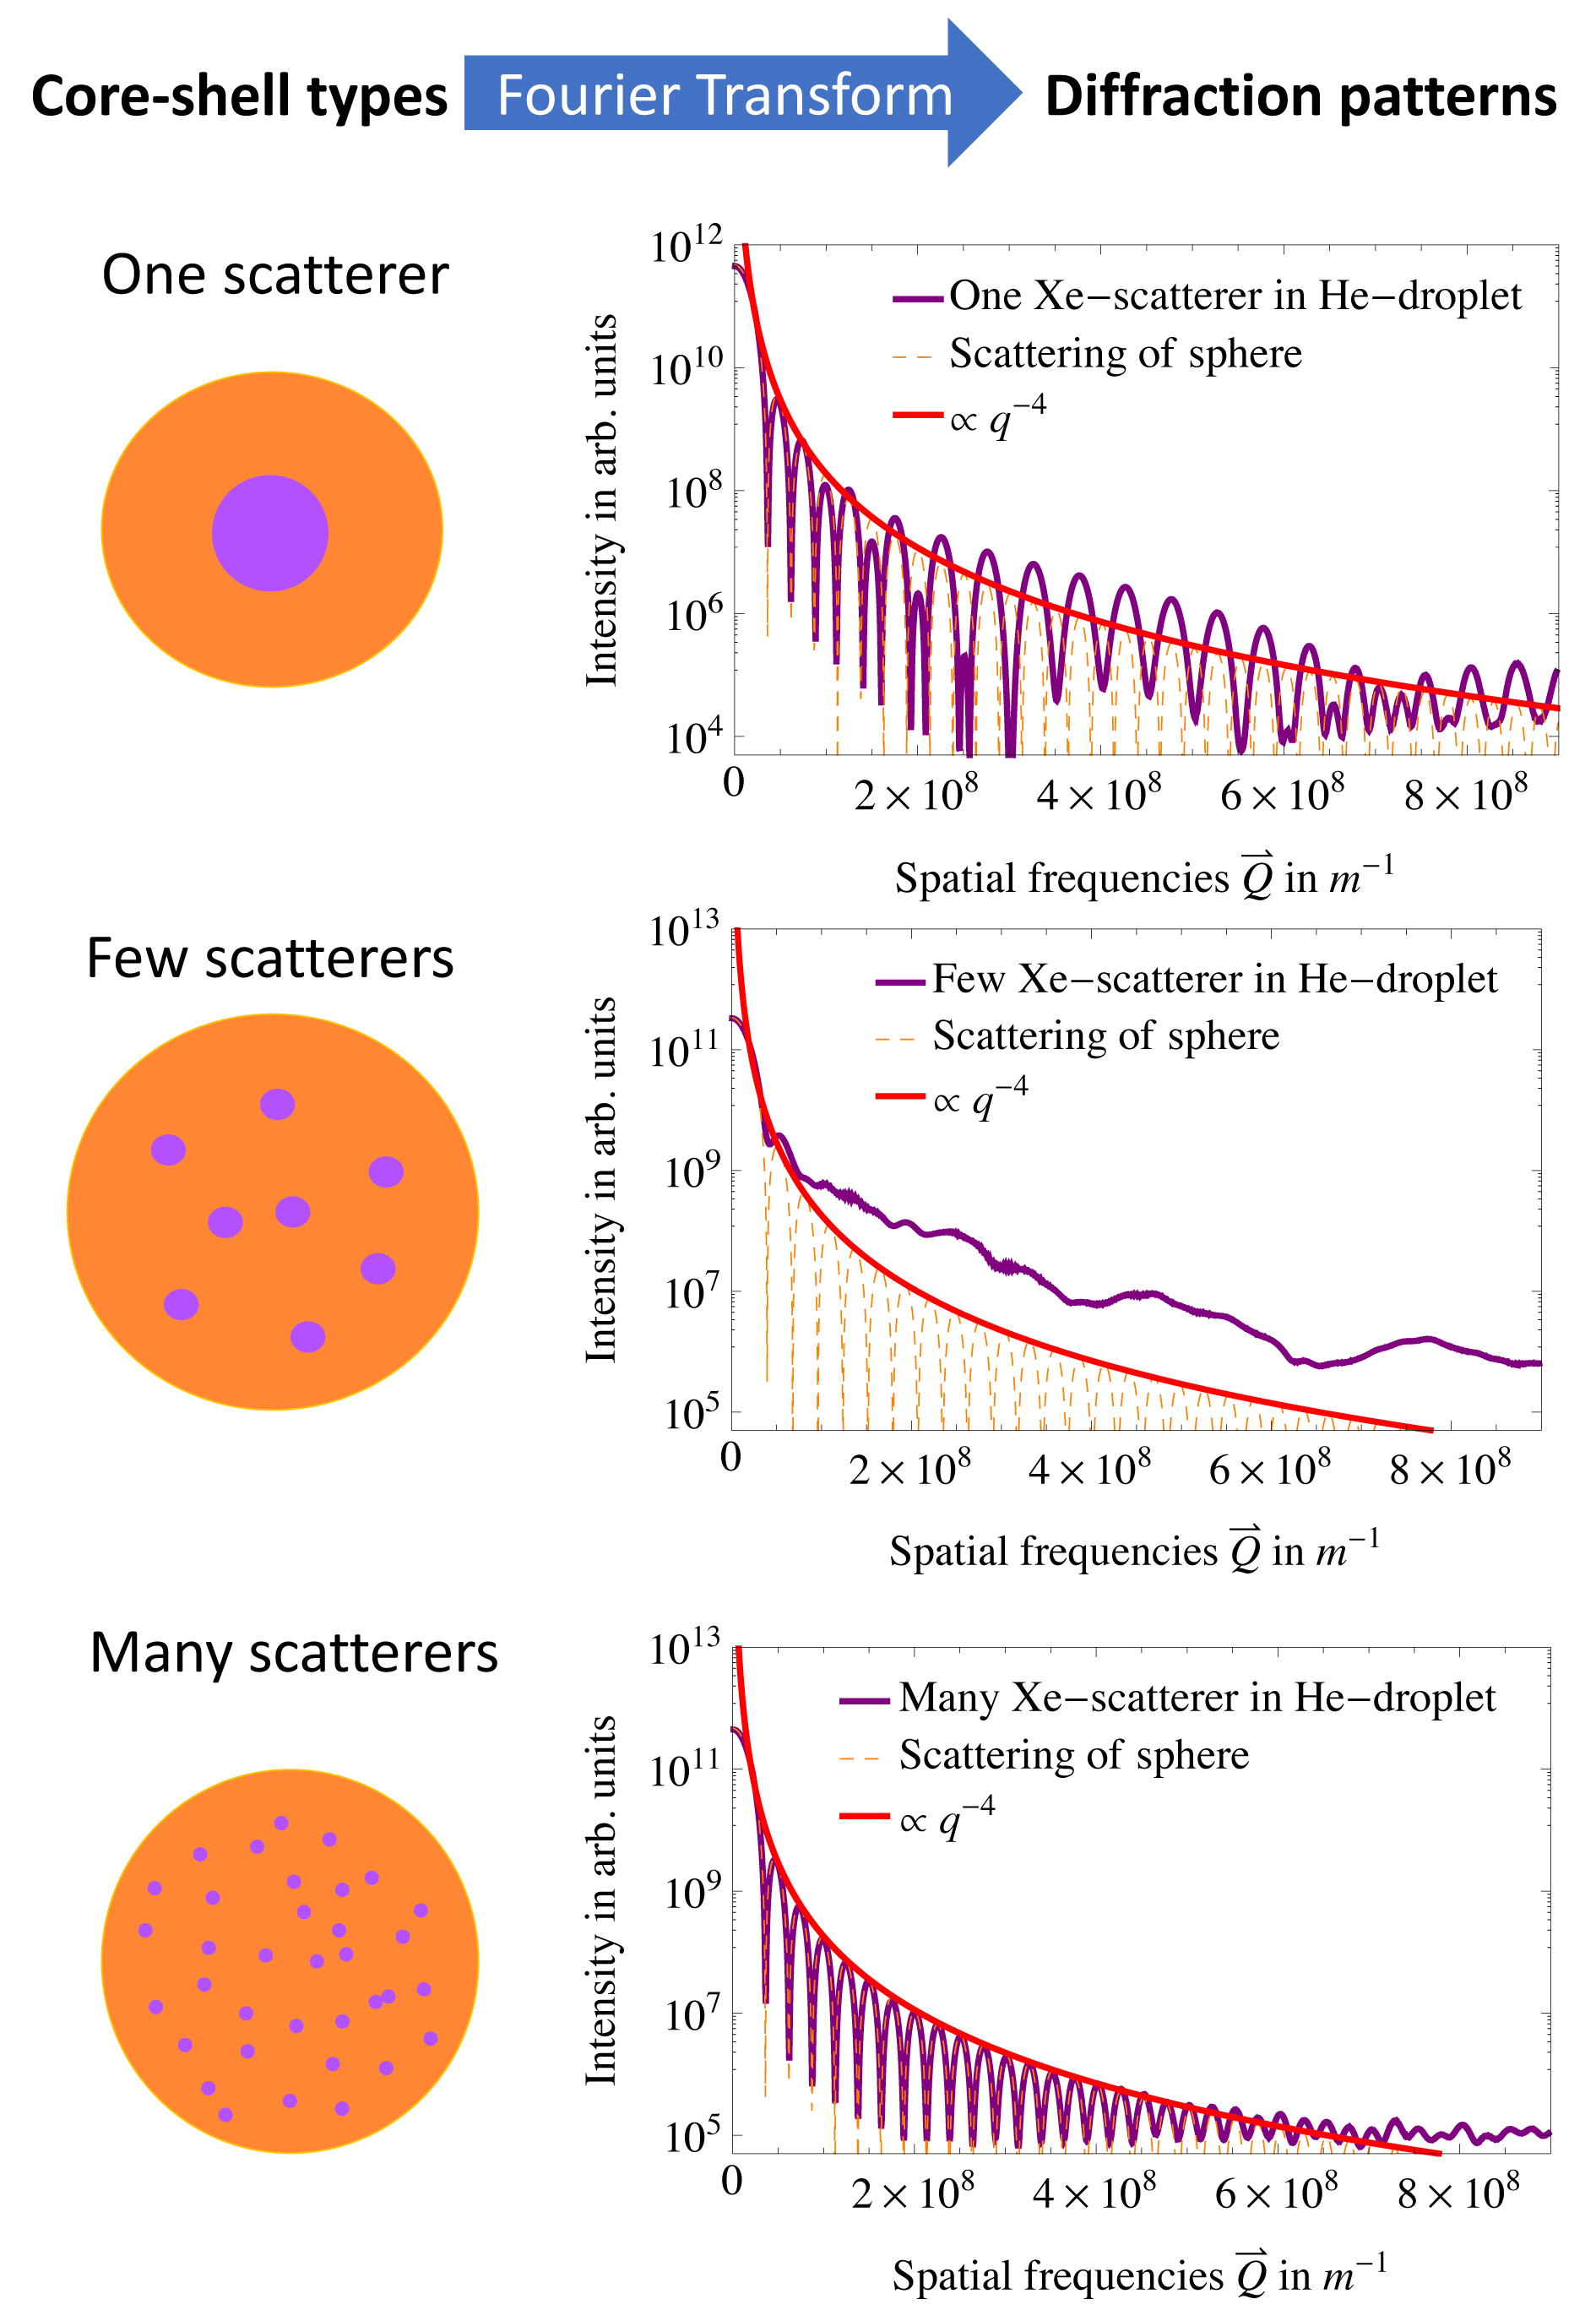
\includegraphics[width=0.82\textwidth]{images/results/plum-pudding.png}
 	\caption[Hypothetical arrangement of Xe-clusters within He-droplets.]{Hypothetical arrangement of xenon atoms in superfluid helium droplets and corresponding 1D diffraction patterns. The He-droplet has a radius of $\sim 125$ nm and the Xe-doping level is $\sim 20\%$. The case of one xenon scattering center $N_{\text{sc}}=1$ (top), few scatterers $N_{\text{sc}}=8$ (middle) and many scatterers $N_{\text{sc}}=100$ (bottom) are shown (left) to illustrate their impact on diffraction pattern (right). The scattering pattern is dominated by the signal from the He-droplet at low $\vec{Q}$-values and at large $\vec{Q}$-values the signal is dominated by the Xe-clusters. This is mostly due to the size of the Xe-clusters; smaller scattering centers are resolved at larger scattering angles.}
 	\label{fig:HeXe-plum-pudding}
\end{figure}
To verify the success of the HeXe-reconstruction, several core-shell arrangements are shown in Figure \ref{fig:HeXe-plum-pudding} along with their Fourier-space representations in 1D. The shown He-droplet has a radius of $r\approx 125$ nm and a constant xenon doping level of $\sim 20\%$ and the figure shows an artistic representation of the simulated real-space core shell systems. These 2D-simulations are described in more detail in Section \ref{sec:2d-simulations}. In the illustration, it becomes obvious that the distribution of the xenon atoms within the He-droplet dominates the scattering pattern, which is due to the Xe-cluster density being $\sim 25.8$ times larger than the density of liquid He-droplets. The purple curve in the one-scatterer case consists of a large modulation in the diffraction image, which comes from the Xe-core and a small, more intense modulation that comes from the He-shell (similar to the orange, dashed line). At low spatial frequencies, the He-droplet dominates the signal on the diffraction image and at large spatial frequencies, the Xe-cluster influence is more prominent. Ultimately, this is related to the size of each cluster and the contributions of their spatial frequencies to modulations in Fourier-space. In the few scatterers case, with $N_{\text{sc}}=8$ scattering centers, the diffraction pattern (purple line) at low spatial frequencies $\vec{Q}$ is still dominated by the He-shell and at large spatial frequencies $\vec{Q}$ by the Xe-cores. However, the diffraction image appears to contain a more complex structure at large $\vec{Q}$-values due to the delocalized scatterers. Also, the average scattering intensity is well above the envelope of the scattering of a sphere (red line) that has been fitted onto the zeroth diffraction order. The location of the few scattering centers plays a lesser role in the 1D projection of the 2D diffraction image, as long as the scattering centers are distributed throughout the He-droplet. In the many scatterers case, $N_{\text{sc}}=100$ scattering centers are randomly distributed within the He-droplet. The Xe-clusters are significantly reduced in size to match the constant xenon doping level of $\sim 20 \%$. For the outer shape, the small clusters appear similar to a constant electron density increase, which is visible at low-to-mid $\vec{Q}$-values. Thus the scattering is practically identical to the scattering of a similar sized sphere (orange, dashed line). Only at large $\vec{Q}$-values that reveal small structures do the Xe-scatterers start to dominate the signal, i.e., signal is above the envelope function of the scattering of the sphere.\\[1\baselineskip]
%
To quantify and estimate the effect of Xe-cluster of a certain size contributing to the spatial frequencies, we can make use of Abbe's criterion \eqref{eq:abbe-criterion} and the wave vector definition \eqref{eq:Q-scattering-angle}. In vacuum, we can write down the minimal resolvable feature size $d$ as
\begin{equation}
d = \frac{2\pi}{\left|\vec{Q_{r}}\right|},
\label{eq:diameter-estimate}
\end{equation}
with $\left|\vec{Q_{r}}\right|$ being the point in reciprocal space, where the signal starts to be dominated by the smaller structures, here the Xe-clusters. We can relate the resolvable feature size $d$ to the radius $r$ of the smaller spherical structures via $d\approx 2 r$. This relation works well for the one-scatterer case $r_{\text{Xe}}\approx 15$ nm. However, as the structures become more complex one has more spatial frequency contributions from not only the smaller structures, i.e., the Xe-cluster, but also the space in between smaller structures and the space from the smaller structures to the boundary of the system, i.e., the He-droplet. Multiple smaller structures thus form a \textit{superstructure}\index{superstructure} that appears larger than its individual components when estimated via Equation \eqref{eq:diameter-estimate}. For the plum-pudding cases the Xe-cluster form superstructures with the He-droplet. This superstructure is $\sim 3$ times larger in the few scatterers case and $\sim 10$ times larger in the many scatterers case than its individual, simulated Xe-cluster components.\\[1\baselineskip]
%The study of diffraction patterns thus gives insight into the heterogeneous core-shell system. Ultimately, the structure of a heterogeneous HeXe-cluster must be understood to further conclude about effects of radiation damage. To study the diffraction pattern of heterogeneous cluster 2D simulations were developed that simulate the electron density of a cluster and then Fourier transform these into Fourier-space. The 2D diffraction images are then projected onto 1D to be compared efficiently. More details about this method can be found in Section \ref{sec:2d-simulations}.\\
%The 2D electron density simulations show that Xe atoms arrange as few randomly orientated clusters within the He-droplet. The data in Figure \ref{fig:HeXe-cluster-60} shows several cases of Xe arrangement within the He-droplet. First, looking at the extreme cases of no Xe-scatterer (n=0) and many small Xe-scatterer $(n=100)$ show vastly different scattering pattern than measured. Only the case of few Xe-scatterer $(n\approx 10)$ reproduces the in the experiment measured data. This approach also allows a precise determination of the Xe-doping level on a shot-to-shot basis as the size of the Xe-cluster within the He-droplet can be adapted to fit the measurement. The overall amount of Xe in the system can be compared to the amount of He and thus a relative doping level is found. In this example, a doping level of XXX was found. This agrees well with the average doping level calculated in Equation \eqref{eq:average-dopant}.\\
%
%
%
% \subsection{Diffraction images of helium cluster}
%%%%%%%%%%%%%%%%%%%%%%%%%%%%%%%%%%%%%%%
%- Work out radiation damage in 1D diffraction images.\\
%- Introduce envelope to show the radiation damage effect - important to compare to HeXe data.\\
%- Eventually subsection for reconstructions.
%%%%%%%%%%%%%%%%%%%%%%%%%%%%%%%%%%%%%%%
%
%
%
\section{Understanding structural damage in the plum-pudding type clusters}\label{sec:helium-xenon-data}
%%%%%%%%%%%%%%%%%%%%%%%%%%%%%%%%%%%%%%
%-Presentation of HeXe data
%%%%%%%%%%%%%%%%%%%%%%%%%%%%%%%%%%%%%%
\begin{figure}
	\centering
		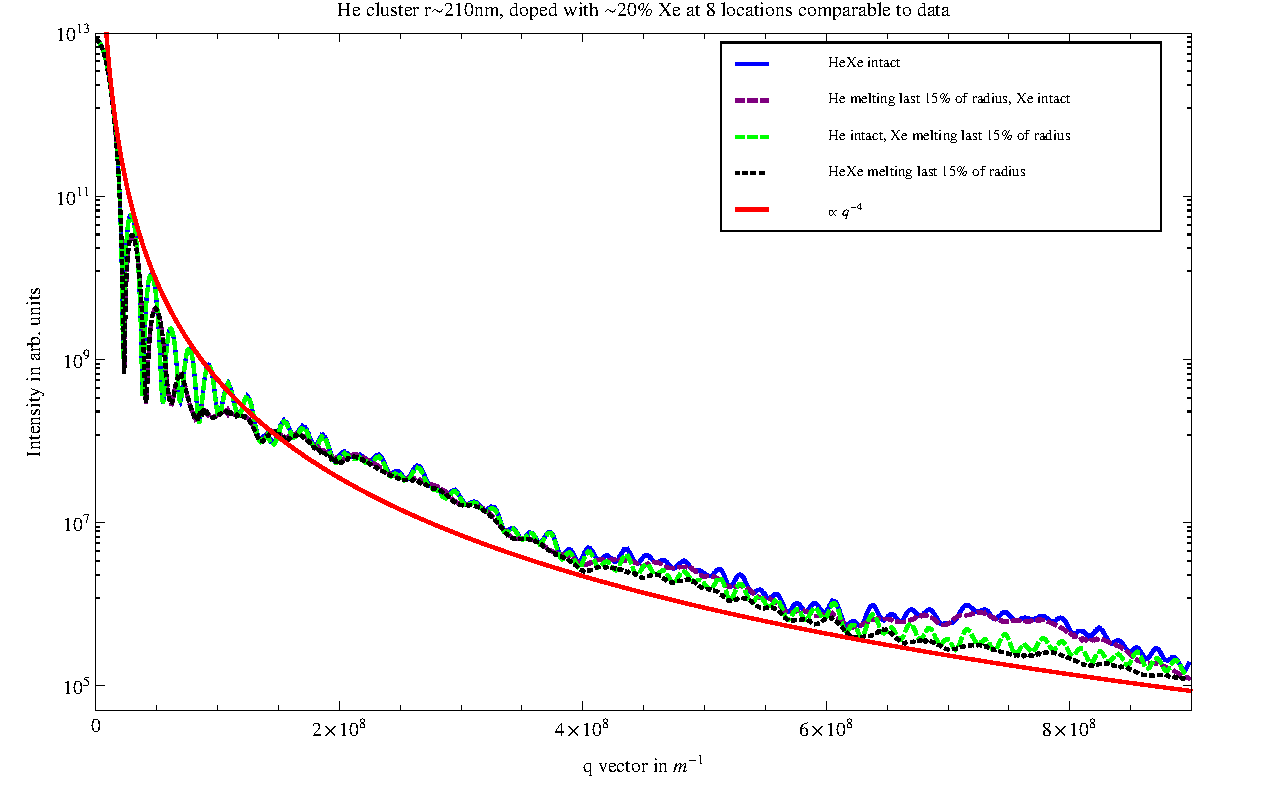
\includegraphics[width=0.80\textwidth]{images/results/simulations-damage-explain.pdf}
	\caption[Simulated structural damage scenarios in HeXe-clusters.]{Diffraction images from 2D electron density simulations that illustrate structural damage in HeXe-cluster. Electron densities as per Figure \ref{fig:HeXe-cluster-60}. In reciprocal space: The blue curve shows the helium droplet as well as Xe-clusters intact. The purple, dashed curve shows an expanding He-droplet, leaving the Xe-clusters intact. The green, dashed curve leaves the He-droplet intact but shows expanding He-clusters. The black, dashed curve shows both cluster types expanding. The red curve is the envelope of the scattering of a sphere fitted to the zeroth order. More in text.}
	\label{fig:simulations-damage-explain}
\end{figure}
Figure \ref{fig:simulations-damage-explain} shows a diffraction pattern from the simulated plum-pudding type electron density shown in Figure \ref{fig:HeXe-cluster-60} that illustrates radiation damage. As described in Section \ref{sec:2d-simulations}, the radiation damage is simulated via an expansion of the outer layers of a sphere. The He-droplet has a radius $r_{\text{He}}=210$ nm and a strong Xe-doping of $\sim 20 \%$ to illustrate the effects of structural damage. The blue, solid curve describes the scenario, where all spheres, i.e., clusters, are intact and no X-ray induced dynamics are present. The purple, dashed curve shows the case where the last \SI{15}{\percent} in units of the He-droplet radius $r$ expand, but the Xe-cluster intact are intact. Conversely, the green, dashed curve shows the effect where the last \SI{15}{\percent} of the radius from Xe-clusters expand, but the He-shell stays intact. Lastly, all spheres are expanding in the last \SI{15}{\percent} of their radii. It can be clearly seen that the expansion of each cluster type effects either low spatial frequencies when the He-droplet is expanding, or high spatial frequencies when the (much smaller) Xe-cluster are expanding. The vast size difference of the Xe-clusters to the He-droplet, wich are $r_{\text{Xe}}=$ \SIlist{25;22;20;18;17;14;14;13.5}{\nano\meter} versus $r_{\text{He}}=\SI{210}{\nano\meter}$, allow a strict separation between the spatial frequency contributions from the He-droplet, e.g., the expanding shell, and the contributions from the Xe-clusters, e.g., the intact cores, in the diffraction pattern analysis.\\[1\baselineskip]
%Now that we have discussed the effects of X-ray induced dynamics, i.e. radiation damage, in Xe-clusters by analyzing single-shot diffraction pattern and time-of-flight mass spectroscopy and also having understood the structure of heterogeneous HeXe cluster as they arrange in a \textit{plum-pudding} type model, where few Xe-scatterer are present in a large He-droplet, we can discuss the diffraction pattern from the pump--probe data of HeXe-clusters. Let us start off by reusing the 2D simulations, described in Section \ref{sec:2d-simulations}, using damaged spheres to investigate the effects onto the diffraction pattern.\\
\begin{figure}
%width=0.49\textwidth
	\centering
		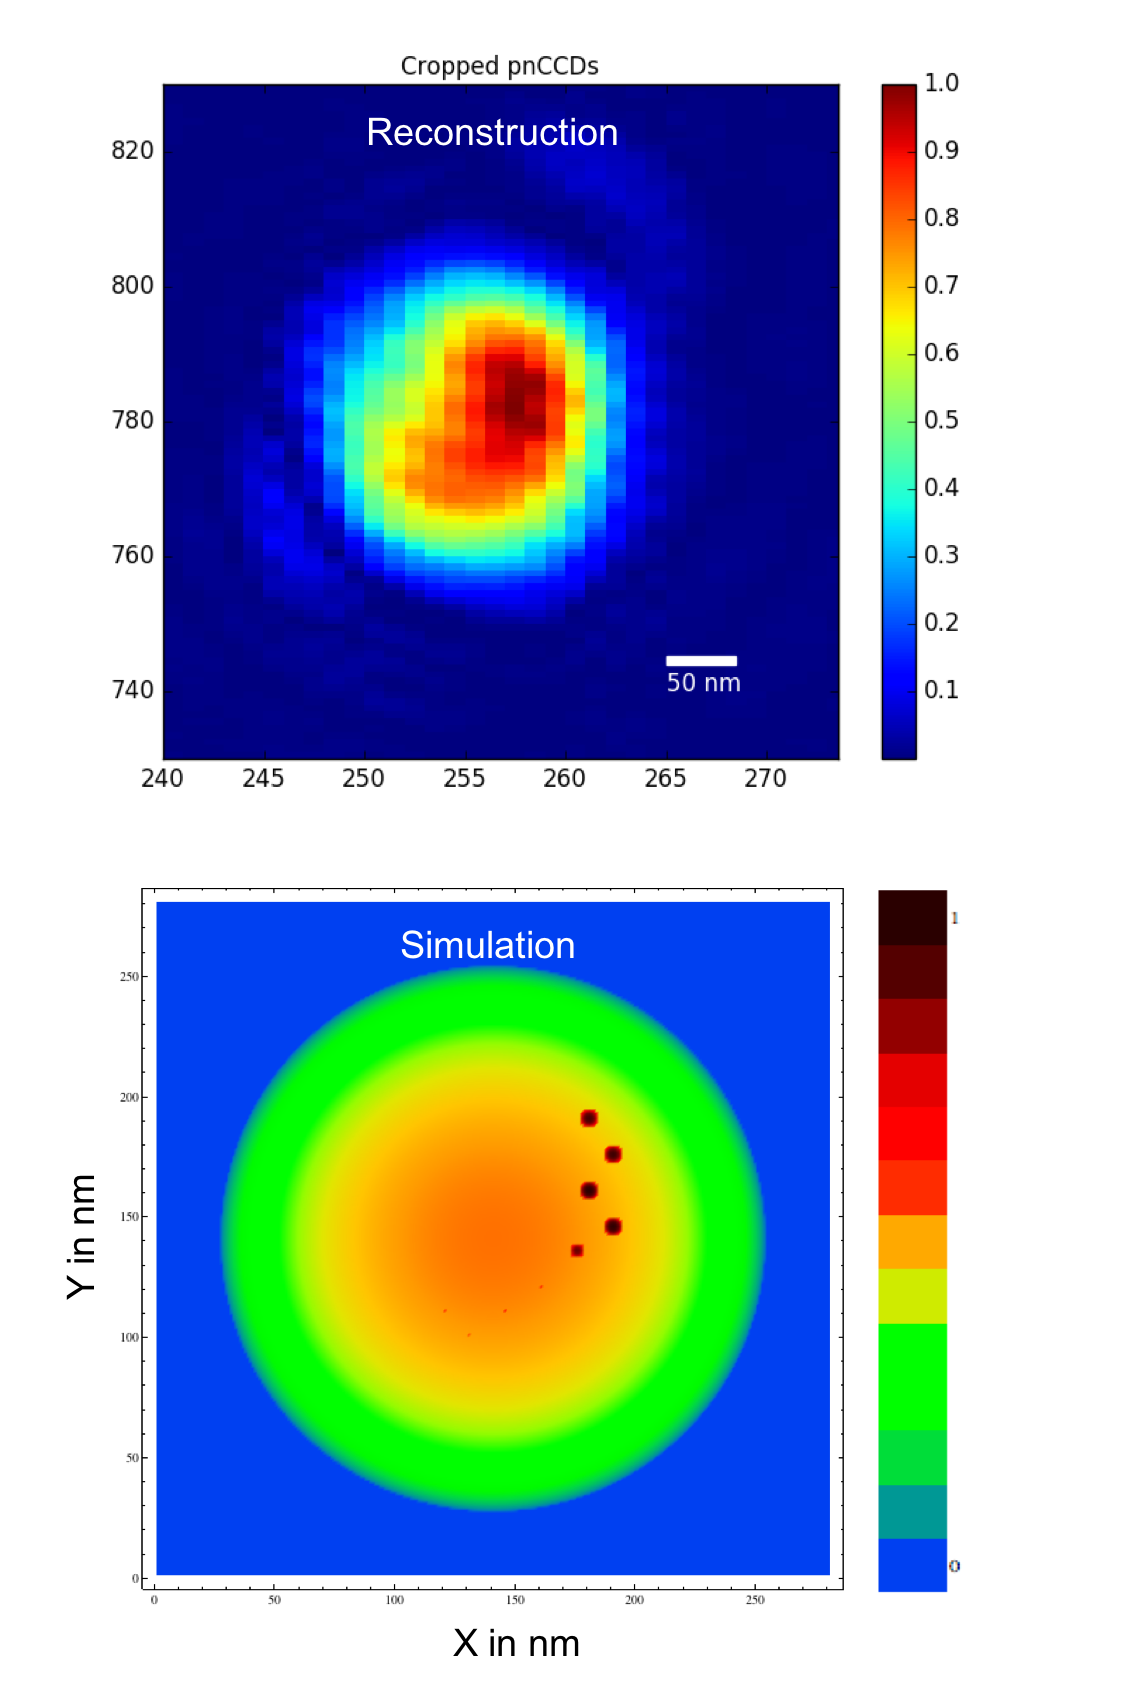
\includegraphics[height=6.0cm]{images/results/HeXe-densities-113-05-doping-and-reconstruction.png}
		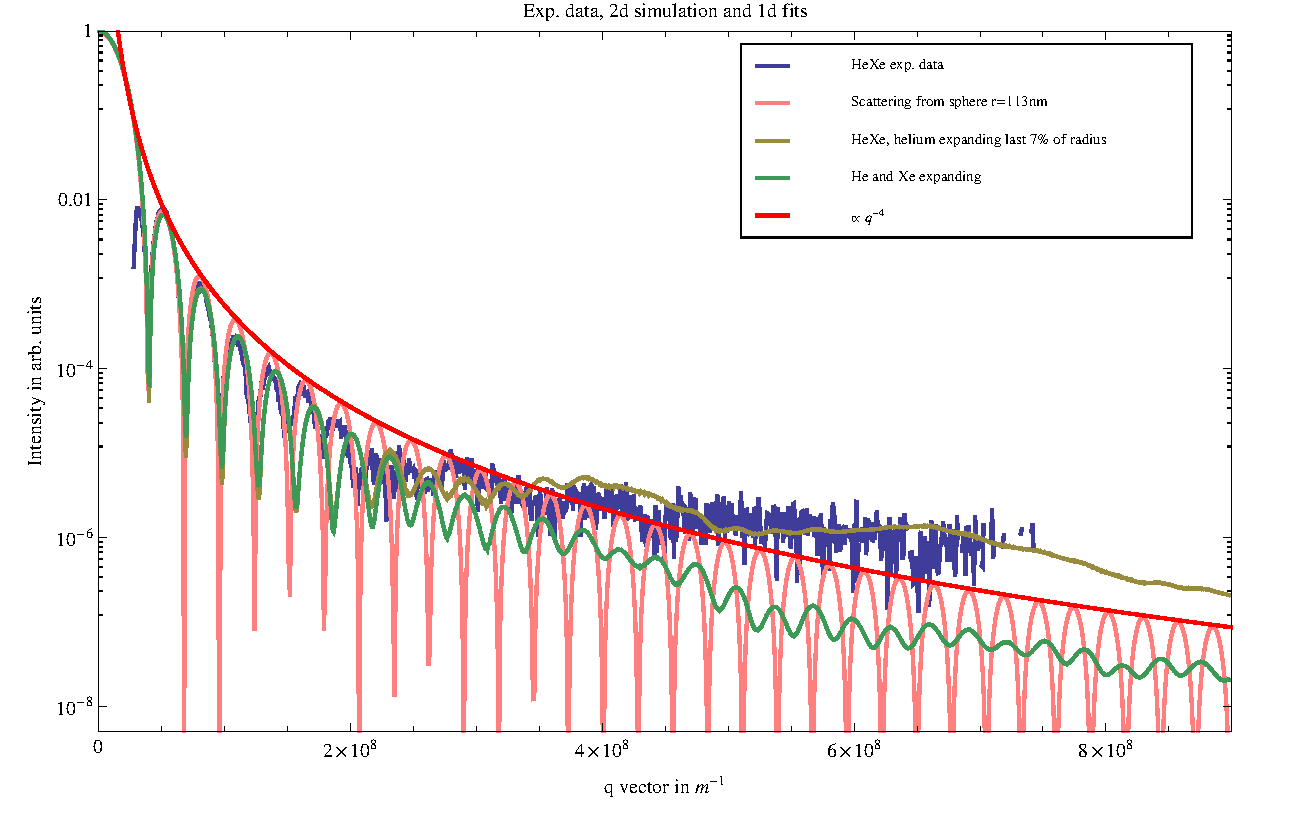
\includegraphics[height=6.0cm]{images/results/HeXe-cluster-113-0-5-doping.pdf}
	\caption[Simulation and exp. data: Structural damage in He-droplet.]{2D simulations fitted to real-space and Fourier-space data. HeXe-arrangement of 2D simulations (bottom left) matches recovered electron densities of a HeXe-cluster (top left). The diffraction pattern (right) shows the 1D-projected experimental data (blue curve) from the same HeXe-cluster with $r_{\text{He}}\approx 113$ nm. This HeXe-cluster was imaged at $\Delta t=800$ fs and undergoes a nanoplasma transition. 2D simulations showcase several damage scenarios; in reciprocal space: Xe-cluster are intact (yellow curve) and Xe-cluster expanding (green curve). The simulations of an expanding He-droplet and intact Xe-cluster fit the experimental data best.}
	\label{fig:HeXe-cluster-113-0.5}
\end{figure}
These insights can be used to compare the 2D-simulations to the measured diffraction patterns. Figure \ref{fig:HeXe-cluster-113-0.5} shows a HeXe-cluster reconstruction, a simulation and corresponding 1D diffraction pattern. This data has been taken at a time delay $\Delta t=800$ fs.The HeXe-cluster has a radius $r_{He}\approx 113$ nm. The dense spots in the reconstruction have been simulated with nine Xe-cluster of radii $r_{Xe}=$ \SIlist{4;4;4;4;3;0.5;0.5;0.5;0.5}{\nano\meter}, thus a $\sim 0.5 \%$ Xe-doping. In the diffraction pattern, the scattering of a sphere with radius $r=113$ nm (pink line) and its envelope (red line) are shown as a comparison. The yellow curve is a simulated diffraction pattern that shows an expanding He-droplet, where the last $7 \%$ of the shell is exponentially expanding, while the Xe-clusters stay intact. The green curve shows the simulated diffraction pattern, where the He-droplet is expanding at the last $7 \%$ of its radius and, to make the effect clear, $90 \%$ of the Xe-clusters outer radii are expanding. The simulations show a very good agreement with the expanding He-droplet at low spatial frequencies $\vec{Q}$. At high frequencies, only the yellow curve that uses intact Xe-clusters in the simulation reproduces the scattering image well. It should be noted, however, that structural damage in the Xe-cluster is still possible, but may not be detectable due to current resolution limitations.
%
%
%
\section{Sacrificial layers: Comparison of structural damage in He- and HeXe-cluster}\label{sec:comparison-of-He-and-HeXe-clusters}
%%%%%%%%%%%%%%%%%%%%
% Start with helium - diff pattern
% Show several HeXe - diff patterns
% Compare...
%%%%%%%%%%%%%%%%%%%%%%
\begin{figure}
	\centering
		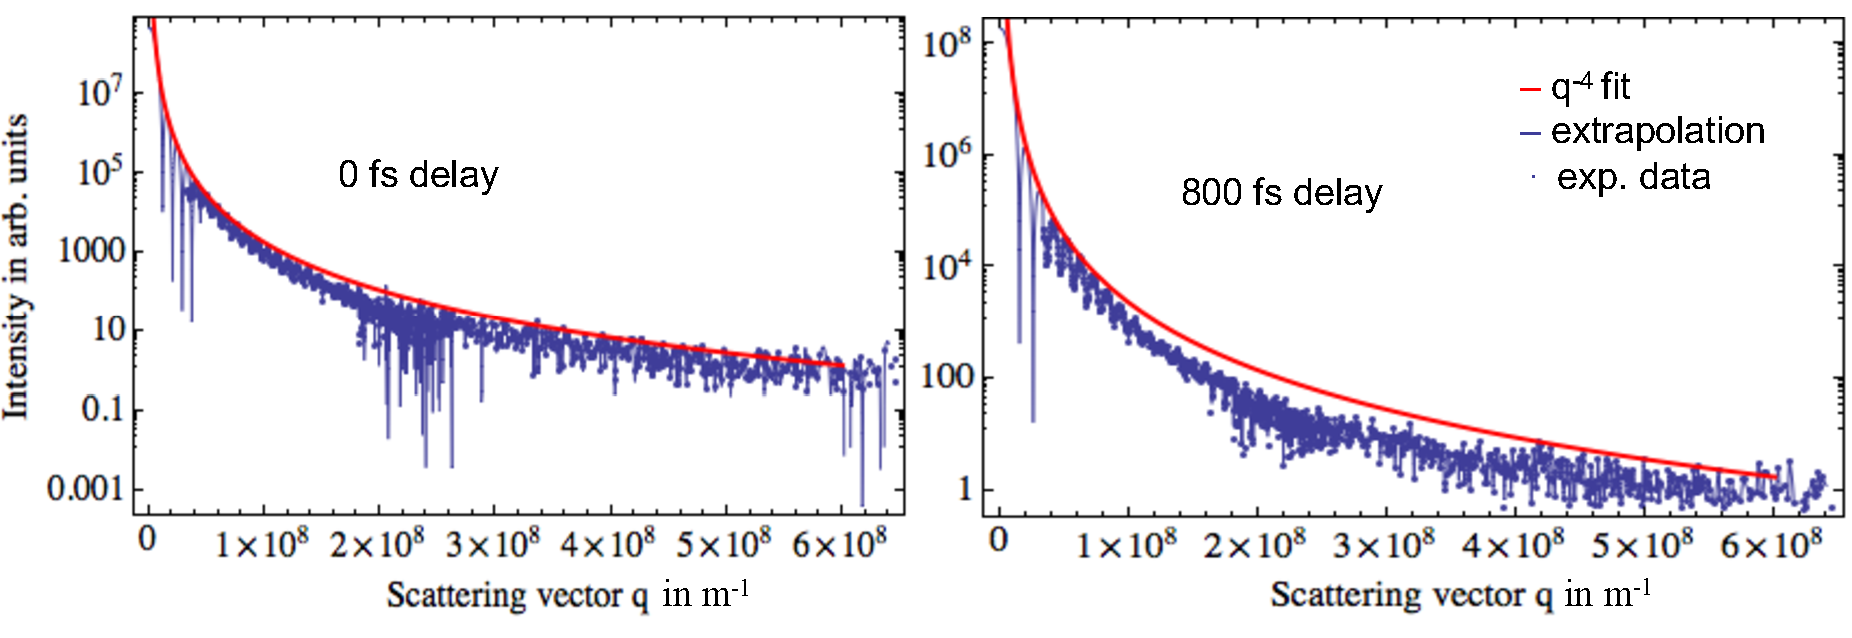
\includegraphics[width=1.00\textwidth]{images/results/He-diffraction-patterns.pdf}
	\caption[Single-shot diffraction images of He-droplets at different time delays]{Single-shot diffraction images of pristine He-droplets at various $\Delta t$ spherically projected into 1D.}
	\label{fig:He-diffraction-patterns}
\end{figure}
Single-shot diffraction images of He-droplets with radii $r_{\text{He}}\approx$ \SIlist{379;302}{\nano\meter}, at time delays $\Delta t=$ \SIlist{0;800}{\femto\second}, respectively, are shown in Figure \ref{fig:He-diffraction-patterns}. For clarity, only the experimental data (blue points), spherical extrapolation at low $\vec{Q}$-values (blue line) and the envelope of the spherical extrapolation function (red line) are shown. At $\Delta t = 0$ fs, the local maxima of the experimental data agree well with the envelope function. This indicates an intact He-droplet, as shown in more detail in Section \ref{sec:xenon-data}. As the time delay is varied to $800$ fs, the diffraction pattern of the droplet shows that the local maxima between $\vec{Q} \approx$ \SIrange[scientific-notation=fixed, fixed-exponent=8]{1e8}{4e8}{\per\meter} are well below the envelope. As shown in section \ref{sec:helium-xenon-data}, this indicates damage.\\[1\baselineskip]
%
\begin{figure}
	\centering
		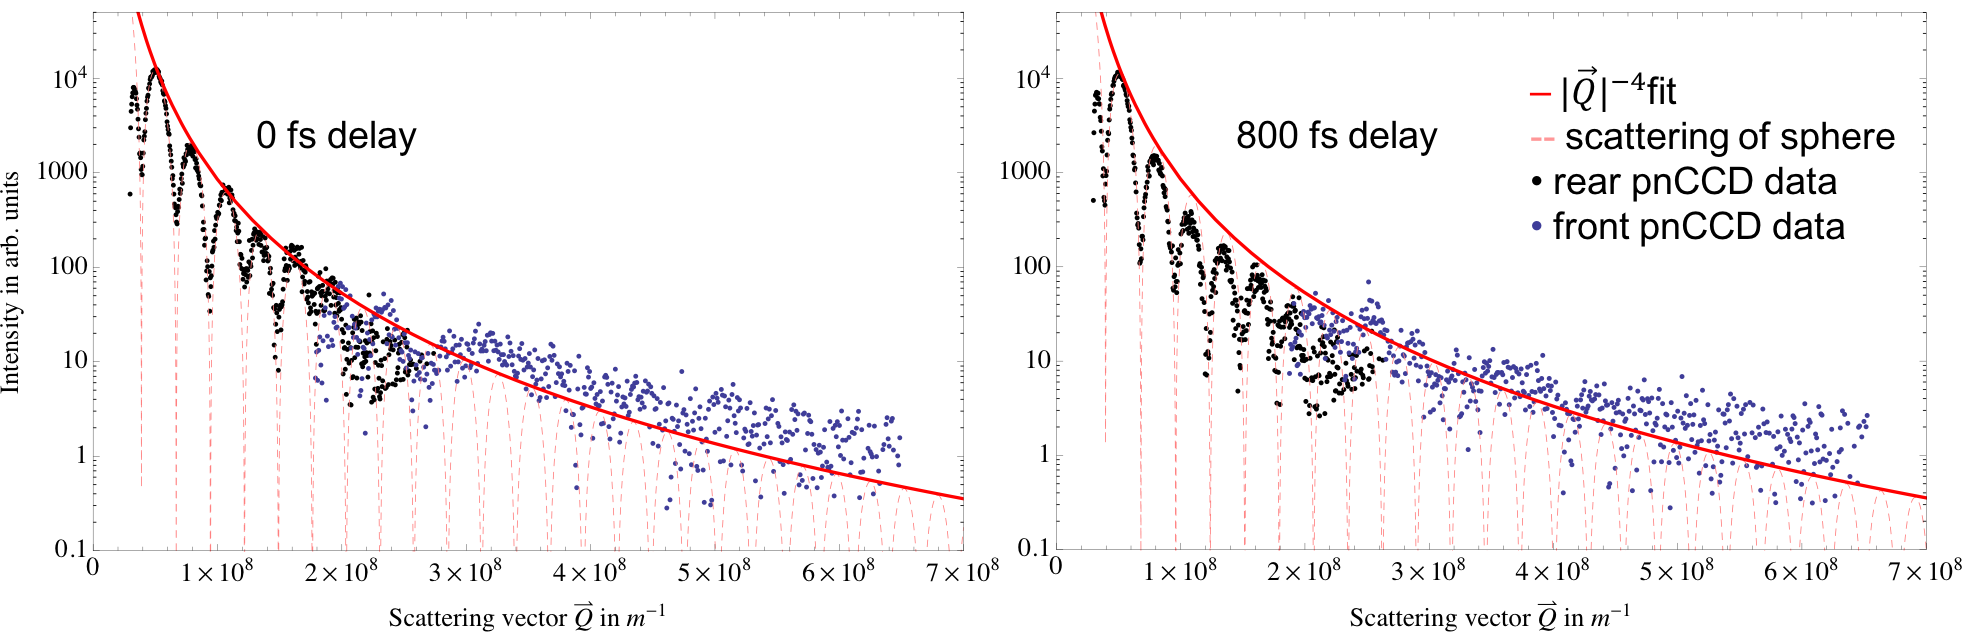
\includegraphics[width=1.00\textwidth]{images/results/HeXe-comparison-0-800-fs.png}
	\caption[Single-shot diffraction patterns of HeXe-cluster at different time delays]{Single-shot diffraction pattern of HeXe-cluster at time delays $\Delta t =$ 
	\SIlist{0;800}{\femto\second}. At $\Delta t=0$ fs, the diffraction pattern follows the scattering pattern of a sphere at low spatial frequencies $\vec{Q}$ but stays well above the envelope function $\vec{Q}^{-4}$ at high spatial frequencies $\vec{Q}$. At $\Delta t=800$ fs, the scattering curve deviates from the scattering pattern of a sphere at low $\vec{Q}$-values indicating damage to the He-shell structure. At large $\vec{Q}$-values, the signal changes little compared to the $\Delta t=0$ fs data indicating intact Xe-cluster, i.e., cores. This suggests that the He-droplet functions as sacrificial shell keeping the Xe-nanoparticles intact. More in text.}
	\label{fig:HeXe-comparison-0-800-fs}
\end{figure}
%
Single-shot diffraction images of HeXe-cluster with radii $r_{\text{He}}\approx$ \SIlist{116;113.5}{\nano\meter}, at time delays $\Delta t =$ \SIlist{0;800}{\femto\second}, respectively, are shown in Figure \ref{fig:HeXe-comparison-0-800-fs}. The experimental data at $\Delta t = 800$ fs is the same as in Figure \ref{fig:HeXe-cluster-113-0.5}. The black dots are data points from the rear pnCCD and the blue dots are data points from the front pnCCD. The pink, dashed curve is the scattering from a sphere fitted to the first order of diffraction and the red curve is its envelope. Here, the differences in the diffraction images as the time delay $\Delta t$ is varied from \SIrange{0}{800}{\femto\second} provide as another indication that helium functions as a sacrificial layer in HeXe-clusters. At $\Delta t=0$ fs, the rear pnCCD data points agree well with the simulated scattering of a sphere, while the data points from the front detector lay well above the scattering envelope function of the sphere. As already discussed, at $\Delta t = 800$ fs the rear pnCCD data points do not agree well with the scattering of a sphere, indicating damage in the He-droplet. However, the blue data points appear to be similar, as in the $\Delta t=0$ fs event.\\[1\baselineskip]
\begin{table}%
\centering
\textbf{Measured scattering / expected scattering}\\
\begin{tabular}{ | c || c | c | }
\hline
	 &\multicolumn{2}{c|}{\textbf{At time delay $\Delta t$}} \\
	\textbf{For sample} & 0 fs  & 800 fs \\ \hline \hline
	Xe-cluster & $0.91\pm \sim 0.1$ & $0.26\pm \sim 0.1$ \\ \hline
	He-droplet & $0.89\pm \sim 0.1$ & $0.65\pm \sim 0.1$ \\ \hline
	HeXe-cluster & $1$ & $1.33\pm \sim 0.3$ \\ \hline
\end{tabular}
\caption[Relative comparison of measured scattering versus expected scattering.]{Relative comparison of measured scattering versus expected scattering for Xe-, He- and HeXe-cluster at large $\vec{Q}$-values. More in text.}
\label{tab:he-vs-xe-vs-hexe-summary}
\end{table}
A more quantitative comparison provides a challenge as each single-shot event has a certain uniqueness attributed to it. However, an attempt to compare the measured scattering versus expected scattering is made in the following and the results are summarized in Table \ref{tab:he-vs-xe-vs-hexe-summary}. The diffraction pattern of a pristine He- or Xe-cluster can be easily compared to the scattering curve of a sphere $f(\vec{Q})$. Hence, we can introduce a function $h(\vec{Q})$ that interpolates between the data points of pristine He- and Xe-cluster. We can calculate a relative difference in the scattering at a certain time delay using the $\tfrac{\sum{h(\vec{Q}})}{\sum{f(\vec{Q})}}|_{\Delta t}^{\text{sample}}$. Since the effect is most visible at large $\vec{Q}$-values, the functions $h$ and $f$ total between $2.8\cdot 10^{8}$ m$^{-1}$ to $6.4\cdot 10^{8}$ m$^{-1}$. For Xe- and He-clusters, we find values close to the expected scattering of similar sized spheres, thus is the measured scattering / expected scattering: $\SI{91}{\percent} |_{\Delta t = 0 \text{fs}}^{\text{Xe}}$ and $\SI{89}{\percent}|_{\Delta t=0 \text{fs}}^{\text{He}}$. As already established, the actual scattering is reduced due to the nanoplasma expansion such that $\SI{26}{\percent} |_{\Delta t = 800 \text{fs}}^{\text{Xe}}$ and $\SI{65}{\percent} |_{\Delta t = 800 \text{fs}}^{\text{Xe}}$. The interpolating function seems to underestimate the actual scattering by $\sim \SI{10}{\percent}$, which gives us an idea of the error of this estimate. Some other error sources such as electronic noise would make up for the underestimate of the interpolating function. HeXe-clusters cannot directly be compared to the scattering of a sphere. However, we may compare similar single-shot events at different time delays. The two single-shot events shown in Figure \ref{fig:HeXe-comparison-0-800-fs} represent similar data points, as they have the same incident beam variable $I_{0}$ in the $I_{0} \left|\vec{Q}\right|^{-4}$ fit and a size difference of only $\sim \SI{2}{\percent}$ at the same source and doping conditions. When comparing the interpolating functions $h(\vec{Q}) |_{\Delta t = 800 \text{fs}}^{\text{HeXe}}/h(\vec{Q}) |_{\Delta t = 0 \text{fs}}^{\text{HeXe}}$ at different time delays $\Delta t$, \SI{33}{\percent} more scattering at large $\vec{Q}$-values is measured. This leads to the conclusion that Xe-clusters exhibit no measurable damage despite the fact that damage in the He-droplet is visible at low spatial frequencies $\vec{Q}$. The error in the estimation originates likely from a varying pickup pattern of Xe-atoms and the error must be at least $\sim \SI{30}{\percent}$.\\[1\baselineskip]
%
Synthesizing, we find a reduction in scattering intensity of $\sim \SI{65}{\percent}$ in Xe-cluster and $\sim \SI{24}{\percent}$ in He-droplets 800 fs after the beginning of the nanoplasma expansion. We attribute this change to damages in the sample\footnote{The actual intensity loss must be larger due to the loss of electrons that is described in Figure \ref{fig:number-of-scatterer}.}. If Xe-clusters are embedded in a He-droplet, no damage is detected in Xe-clusters 800 fs after the nanosample has been pumped by LCLS, although the He-droplet shows damage. The He-droplet appears to shed atomic layers, which transports energy away from the Xe-clusters and enables them to exhibit no measurable damage patterns that were discussed in Section \ref{sec:helium-xenon-data}.
%
%
%
%\subsection{Time-of-flight data of helium-xenon core-shell systems}
%%%%%%%%%%%%%%%%%%%%%%%%%%%%%%%%%%%%%%%%%%%%%%%%%%%
%- Show dynamics of XeHe data in tof trace.\\
%- More hefty nanoplasma expansion in HeXe than in raw He.\\
%- Complement with simulations from Phay.
%%%%%%%%%%%%%%%%%%%%%%%%%%%%%%%%%%%%%%%%%%%%%%%%%%%
%
%
%
%\subsection{Diffraction images of helium-xenon core shell systems}
%%%%%%%%%%%%%%%%%%%%%%%%%%%%%%%%%%%%%%%%%%%%%%%%%
%- Discuss diffraction images\\
%- Show how scattering intensity drops from He signal but not from Xe signal.\\
%- Eventually subsection for reconstructions.
%%%%%%%%%%%%%%%%%%%%%%%%%%%%%%%%%%%%%%%%%%%%%%%%%
%
%
%
%\subsection{Core-shell system considerations}
%
%
%
%\section{Static data}\label{sec:static}
%%%%%%%%%%%%%%%%%%%%%%%%%%%%%%%%%%%%%%%%%%
%-Include in other studies? Or appendix?
%%%%%%%%%%%%%%%%%%%%%%%%%%%%%%%%%%%%%%%%%%%%
%
%
%
%\section{Discussion and conclusion of the X-ray pump--X-ray probe study}
%%%%%%%%%%%%%%%%%%%%%%%%%%%%%%%%%%%%%%%%
%- Conclusion where the results are compared to each other\\
%- This experiment shows that heterogeneous clusters, as in tampered layers, do inhibit radiation damage of the sample target while the sacrificial layer undergoes a rapid nanoplasma transition.
%%%%%%%%%%%%%%%%%%%%%%%%%%%%%%%%%%%%%%%%%%
%The X-ray pump--X-ray probe study reveals some induced dynamics in Xe- and HeXe-cluster. In pristine Xe-cluster, we observe the nanoplasma expansion in the diffraction patternsa nd we can compare the results to other pump--probe studies using optical pump laser. The absorbed energy by the Xe-cluster is comparable in the optical to X-ray study (TBD), which is most relevant for the extend of the nanoplasma expansion. The time-of-flight spectroscopy reveals a to optical laser hidden resonance that is likely due to relaxation processes in the highly excited atoms. As an inner shell electron is ionized a chemical shift changes the ionization potentials and dynamic relaxation processes allow the absorption of more photons at certain stages \citep{Ho-2014-PRL}.\\
%Heterogeneous HeXe-cluster, doped using the pickup-principle, arrange in a plum-pudding type model, where Xe atoms form few Xe-cluster within one large (superfluid) He-droplet. 2D-simulations furthermore show that the X-ray induced dynamics in HeXe-cluster manifest only in the He-droplet.
%
%
%